% Options for packages loaded elsewhere
\PassOptionsToPackage{unicode}{hyperref}
\PassOptionsToPackage{hyphens}{url}
\PassOptionsToPackage{dvipsnames,svgnames,x11names}{xcolor}
%
\documentclass[
]{agujournal2019}

\usepackage{amsmath,amssymb}
\usepackage{iftex}
\ifPDFTeX
  \usepackage[T1]{fontenc}
  \usepackage[utf8]{inputenc}
  \usepackage{textcomp} % provide euro and other symbols
\else % if luatex or xetex
  \usepackage{unicode-math}
  \defaultfontfeatures{Scale=MatchLowercase}
  \defaultfontfeatures[\rmfamily]{Ligatures=TeX,Scale=1}
\fi
\usepackage{lmodern}
\ifPDFTeX\else  
    % xetex/luatex font selection
\fi
% Use upquote if available, for straight quotes in verbatim environments
\IfFileExists{upquote.sty}{\usepackage{upquote}}{}
\IfFileExists{microtype.sty}{% use microtype if available
  \usepackage[]{microtype}
  \UseMicrotypeSet[protrusion]{basicmath} % disable protrusion for tt fonts
}{}
\makeatletter
\@ifundefined{KOMAClassName}{% if non-KOMA class
  \IfFileExists{parskip.sty}{%
    \usepackage{parskip}
  }{% else
    \setlength{\parindent}{0pt}
    \setlength{\parskip}{6pt plus 2pt minus 1pt}}
}{% if KOMA class
  \KOMAoptions{parskip=half}}
\makeatother
\usepackage{xcolor}
\setlength{\emergencystretch}{3em} % prevent overfull lines
\setcounter{secnumdepth}{5}
% Make \paragraph and \subparagraph free-standing
\ifx\paragraph\undefined\else
  \let\oldparagraph\paragraph
  \renewcommand{\paragraph}[1]{\oldparagraph{#1}\mbox{}}
\fi
\ifx\subparagraph\undefined\else
  \let\oldsubparagraph\subparagraph
  \renewcommand{\subparagraph}[1]{\oldsubparagraph{#1}\mbox{}}
\fi


\providecommand{\tightlist}{%
  \setlength{\itemsep}{0pt}\setlength{\parskip}{0pt}}\usepackage{longtable,booktabs,array}
\usepackage{calc} % for calculating minipage widths
% Correct order of tables after \paragraph or \subparagraph
\usepackage{etoolbox}
\makeatletter
\patchcmd\longtable{\par}{\if@noskipsec\mbox{}\fi\par}{}{}
\makeatother
% Allow footnotes in longtable head/foot
\IfFileExists{footnotehyper.sty}{\usepackage{footnotehyper}}{\usepackage{footnote}}
\makesavenoteenv{longtable}
\usepackage{graphicx}
\makeatletter
\def\maxwidth{\ifdim\Gin@nat@width>\linewidth\linewidth\else\Gin@nat@width\fi}
\def\maxheight{\ifdim\Gin@nat@height>\textheight\textheight\else\Gin@nat@height\fi}
\makeatother
% Scale images if necessary, so that they will not overflow the page
% margins by default, and it is still possible to overwrite the defaults
% using explicit options in \includegraphics[width, height, ...]{}
\setkeys{Gin}{width=\maxwidth,height=\maxheight,keepaspectratio}
% Set default figure placement to htbp
\makeatletter
\def\fps@figure{htbp}
\makeatother
% definitions for citeproc citations
\NewDocumentCommand\citeproctext{}{}
\NewDocumentCommand\citeproc{mm}{%
  \begingroup\def\citeproctext{#2}\cite{#1}\endgroup}
\makeatletter
 % allow citations to break across lines
 \let\@cite@ofmt\@firstofone
 % avoid brackets around text for \cite:
 \def\@biblabel#1{}
 \def\@cite#1#2{{#1\if@tempswa , #2\fi}}
\makeatother
\newlength{\cslhangindent}
\setlength{\cslhangindent}{1.5em}
\newlength{\csllabelwidth}
\setlength{\csllabelwidth}{3em}
\newenvironment{CSLReferences}[2] % #1 hanging-indent, #2 entry-spacing
 {\begin{list}{}{%
  \setlength{\itemindent}{0pt}
  \setlength{\leftmargin}{0pt}
  \setlength{\parsep}{0pt}
  % turn on hanging indent if param 1 is 1
  \ifodd #1
   \setlength{\leftmargin}{\cslhangindent}
   \setlength{\itemindent}{-1\cslhangindent}
  \fi
  % set entry spacing
  \setlength{\itemsep}{#2\baselineskip}}}
 {\end{list}}
\usepackage{calc}
\newcommand{\CSLBlock}[1]{\hfill\break\parbox[t]{\linewidth}{\strut\ignorespaces#1\strut}}
\newcommand{\CSLLeftMargin}[1]{\parbox[t]{\csllabelwidth}{\strut#1\strut}}
\newcommand{\CSLRightInline}[1]{\parbox[t]{\linewidth - \csllabelwidth}{\strut#1\strut}}
\newcommand{\CSLIndent}[1]{\hspace{\cslhangindent}#1}

\usepackage{booktabs}
\usepackage{caption}
\usepackage{longtable}
\usepackage{colortbl}
\usepackage{array}
\usepackage{url} %this package should fix any errors with URLs in refs.
\usepackage{lineno}
\usepackage[inline]{trackchanges} %for better track changes. finalnew option will compile document with changes incorporated.
\usepackage{soul}
\linenumbers
\makeatletter
\@ifpackageloaded{caption}{}{\usepackage{caption}}
\AtBeginDocument{%
\ifdefined\contentsname
  \renewcommand*\contentsname{Table of contents}
\else
  \newcommand\contentsname{Table of contents}
\fi
\ifdefined\listfigurename
  \renewcommand*\listfigurename{List of Figures}
\else
  \newcommand\listfigurename{List of Figures}
\fi
\ifdefined\listtablename
  \renewcommand*\listtablename{List of Tables}
\else
  \newcommand\listtablename{List of Tables}
\fi
\ifdefined\figurename
  \renewcommand*\figurename{Figure}
\else
  \newcommand\figurename{Figure}
\fi
\ifdefined\tablename
  \renewcommand*\tablename{Table}
\else
  \newcommand\tablename{Table}
\fi
}
\@ifpackageloaded{float}{}{\usepackage{float}}
\floatstyle{ruled}
\@ifundefined{c@chapter}{\newfloat{codelisting}{h}{lop}}{\newfloat{codelisting}{h}{lop}[chapter]}
\floatname{codelisting}{Listing}
\newcommand*\listoflistings{\listof{codelisting}{List of Listings}}
\makeatother
\makeatletter
\makeatother
\makeatletter
\@ifpackageloaded{caption}{}{\usepackage{caption}}
\@ifpackageloaded{subcaption}{}{\usepackage{subcaption}}
\makeatother
\ifLuaTeX
  \usepackage{selnolig}  % disable illegal ligatures
\fi
\usepackage{bookmark}

\IfFileExists{xurl.sty}{\usepackage{xurl}}{} % add URL line breaks if available
\urlstyle{same} % disable monospaced font for URLs
\hypersetup{
  pdftitle={Distinct functional responses of consumers and their producers to climate drive mutualistic network asymmetry},
  pdfauthor={Gabriel Munoz; Paul Savary; W. Daniel Kissling; JP Lessard},
  pdfkeywords={Climate change, Frugivory, Interaction diversity, Network
specialization, Seed dispersal},
  colorlinks=true,
  linkcolor={blue},
  filecolor={Maroon},
  citecolor={Blue},
  urlcolor={Blue},
  pdfcreator={LaTeX via pandoc}}

\journalname{Manuscript in Progress}

\draftfalse

\begin{document}
\title{Distinct functional responses of consumers and their producers to
climate drive mutualistic network asymmetry}

\authors{Gabriel Munoz\affil{1}, Paul Savary\affil{1}, W. Daniel
Kissling\affil{2}, JP Lessard\affil{1}}
\affiliation{1}{Concordia University, }\affiliation{2}{University of
Amsterdam, }
\correspondingauthor{Gabriel Munoz}{gabrielmunoz1891@gmail.com}


\begin{abstract}
\textbf{Aim:} Functional traits are often used to infer the ecological
processes that determine the composition of species assemblages.
However, most trait-based approaches to infer community assembly
processes focus on a single trophic level. Owing to the matching of
traits facilitating interactions between resource and consumer
assemblages, the functional trait diversity of different trophic levels
is expected to covary in space. However, differential response of
consumers and producers to environmental gradients can cause a
decoupling of functional diversity between trophic levels, which we coin
functional trophic asymmetry. Here, we develop a metric to quantify
functional trophic asymmetry (FTA) and use it to infer the processes
underpinning multitrophic community assembly, and explore the role of
these processes in shaping the topology of ecological networks.

\textbf{Location:} Neotropics.

\textbf{Time period:} Present.

\textbf{Major taxa:} Mammalian frugivores and palms.

\textbf{Methods:} We use digitally available data on the functional
traits, pairwise mutualistic interactions, and geographic distributions
of consumers (mammalian frugivores) and their producers (palms) to
quantify functional trophic asymmetry for species occurring in the
Neotropics. To cover major data gaps between species-level trait and
interaction data, we train machine learning models to generate synthetic
network data. We then use linear regression models to relate functional
asymmetry to variation in climate, and to assess the influence of
functional asymmetry on network specialization.

\textbf{Results:} Our approach generated probabilistic networks across
1,072 grid cells in the Neotropics, revealing networks with a clearly
defined modular structure and substantial differences in their
functional richness across trophic levels. Functional trophic asymmetry
increases from regions of the Neotropics with low precipitation
seasonality to regions with high precipitation seasonality. Along this
same climatic gradient, network specialization is positively related to
functional trophic asymmetry.

\textbf{Main conclusions:} Our results further suggest that mutualistic
interactions between palms and mammals are mediated by matching traits
and taxonomic overlap as a key assembly process at the regional scale.
We conclude that increased warming and seasonal shifts in precipitation
caused by global climate change could disproportionately impact
specialist species while increasing functional trophic asymmetry in
ecological networks.
\end{abstract}

\section*{Plain Language Summary}
This study explores how differences in functional traits between
co-occurring species assemblages of consumer and producers affect
ecological network assembly in the Neotropics. By focusing on mammalian
frugivores and palms as a case study, we developed a novel metric
functional trophic asymmetry (FTA) to measure mismatches in trait
diversity between trophic levels. Using machine learning and statistical
models to agument spatially sparse data on species interactions, we
found that FTA increases in areas with high precipitation seasonality
and leads to more specialized ecological networks. The results suggest
that climate change could disproportionately impact specialist species
and increase FTA, altering the structure of species interactions in
these ecosystems.



\section{Introduction}\label{introduction}

Ecologists often examine patterns of functional trait diversity to
investigate community assembly processes (Ackerly, 2003; Kraft et al.,
2015). To date, however, trait-based approaches in ecology often focus
on a single trophic level, whereas approaches that consider multiple
trophic levels remain rare (Lavorel et al., 2013; Seibold et al., 2018).
An approach that considers processes operating within and between
trophic levels is necessary to better understand the assembly of
multitrophic communities(Allesina et al., 2008; Marjakangas et al.,
2022; Saravia et al., 2022). Moreover, considering trophic interactions
while studying community assembly could shed new light on processes
underpinning ecological networks (Allesina et al., 2008) .

Classical approaches to study community assembly rely on the concept of
environmental filtering, sorting or selection, where density independent
conditions constrain the functional richness of species assemblages
(HilleRisLambers et al., 2012; Kraft et al., 2015; Laliberté \&
Legendre, 2010; Villéger et al., 2008). Functional richness refers to
the variability and relative frequency of different functional traits
observed in a community. It is often used to estimate the strength of
selection imposed by the environment (Kraft et al., 2008, 2015; Kraft \&
Ackerly, 2010). High functional richness can indicate weak environmental
selection whereas low functional richness can indicate strong selection
(Halpern \& Floeter, 2008; Kraft et al., 2008; Paine et al., 2011). In a
multitrophic context, the effects of environmental selection can cascade
across trophic levels such that selection on consumer traits can shape
the functional richness of their resources, modulated by their degree of
reciprocal dependency or co-evolution (Guzman et al., 2019; Lavorel et
al., 2013). Moreover, the same environmental gradient could exert
selective pressures of different strength on communities at distinct
trophic levels (Marjakangas et al., 2022). Differences in the strength
of selective pressure among trophic levels could then possibly constrain
the structure or topologies of trophic networks (Blüthgen et al., 2007;
Dehling et al., 2020; Schleuning et al., 2012).

Inferring the relative strength of environmental selection between
trophic levels requires using high-dimensional approaches that are able
to deal with sparse observations for a large number of species (Rohr et
al., 2010; Strydom et al., 2022). We introduce the concept of functional
trophic asymmetry (FTA), which allows inferring the relative influence
of environmental selection and trait matching on the composition of
multitrophic assemblages \href{Figure\%201}{(Figure 1)}. FTA is the
difference in the richness of interaction-relevant traits between
trophic levels in a multitrophic network. FTA can occur because traits
mediating species interactions (i.e., interaction niches) across trophic
levels can also mediate the responses of species to their abiotic
environment (i.e.~environmental niches) (Dehling et al., 2020; McCain \&
King, 2014; Moretti \& Legg, 2009; Nagy et al., 2018). As an example,
plant seed size determine the outcome of animal-mediated seed dispersal
(Donoso et al., 2017, 2020) as well as physiological limits, such as
tolerances of plant seedlings to desiccation (Hoekstra et al., 2001).
High FTA could indicate differences in the strength of environmental
selection over the interaction niches of distinct trophic levels within
a multitrophic species assemblage. Alternatively, low FTA could indicate
that the strength of the environment selection shaping interaction
niches is similar between trophic levels, e.g.~equally weak or equally
strong (Marjakangas et al., 2022). When interactions between producers
and consumers are mutualistic, low FTA could also emerge under strong
trait matching and therefore indicate the influence of trait-coevolution
during multitrophic community assembly (Albrecht et al., 2018; Dehling
et al., 2014). By studying spatial variation in functional trophic
asymmetry along environmental gradients, we could possibly identify the
conditions promoting environmentally versus cross-trophic interaction-
driven community assembly (Bello et al., 2023; Schleuning et al., 2020).

Frameworks linking multitrophic functional diversity to network topology
along broad-scale environmental gradients are crucial to understand the
effects of global change on biodiversity and ecosystem function (Bello
et al., 2023; Dehling, 2018; Schleuning et al., 2014, 2020, 2023).
Functional responses of consumer and producer assemblages to climate
influence functional richness at the level of the multitrophic community
(Garcı́a et al., 2018). Because some of these traits are involved in
interactions across trophic levels, the filtering of traits along
environmental gradients could constrain the number of unique
interactions and therefore, network topology (Albrecht et al., 2018;
Emer et al., 2020; Marjakangas et al., 2022). As an example, low
multitrophic functional richness could influence emergent patterns in
network structure such as the specialization of multispecies
interactions by limiting the relative availability of interaction
partners across trophic levels (Blüthgen et al., 2006, 2007). While high
levels of network specialization represent networks predominantly made
of ``one-to-one'' interactions, low levels of network specialization
represent networks with species showing predominantly ``one-to-many''
interactions (Blüthgen et al., 2006; Blüthgen \& Klein, 2011) (Figure
1B). One highly expected outcome is that when functional trophic
asymmetry is high, networks will have low specialization. For example,
take a plant community exhibiting a low richness of flower displays and
which is associated with a bee community (pollinators) exhibiting a wide
variety of proboscis lengths. These plants are unlikely to form
``one-to-one'' interactions with only a subset of bee species that have
matching proboscis length. Otherwise, non-matching pollinators would
have no food resource and be extirpated. By partitioning deviations from
expected FTA and network specialization relationships with null models,
one can separate the relative influences of processes operating between
trophic levels (e.g.~trait matching) and those within trophic levels
(e.g.~environmental selection) in network assembly (Marjakangas et al.,
2022). However, the relationship between network specialization and
functional trophic asymmetry has not been fully explored.

Preserving mutualistic interactions between palms and their mammalian
frugivores is important to sustain biodiversity and ecosystem function
in the tropics (Bogoni et al., 2020; Marques Dracxler \& Kissling,
2022). Mammalian frugivores facilitate the dispersal of palm fruits,
which helps to prevent local extinctions amid disturbance and to
maintain biodiversity in these ecological networks (Acevedo-Quintero,
Saldaña-Vázquez, et al., 2020; Dehling, 2018; Messeder et al., 2020).
Exploring patterns of co-variation in the functional richness of palm
and frugivore assemblages along environmental gradients is a first step
in this direction. Here, we ask (1) which climatic variable(s) best
explains variation in the functional richness of palms vs mammal
frugivores, (2) whether differences in these relationships lead to
functional trophic asymmetry, (3) where does functional asymmetry peaks
in the Neotropics and (4) whether asymmetry relates to network
specialization.

\begin{figure}

{\centering 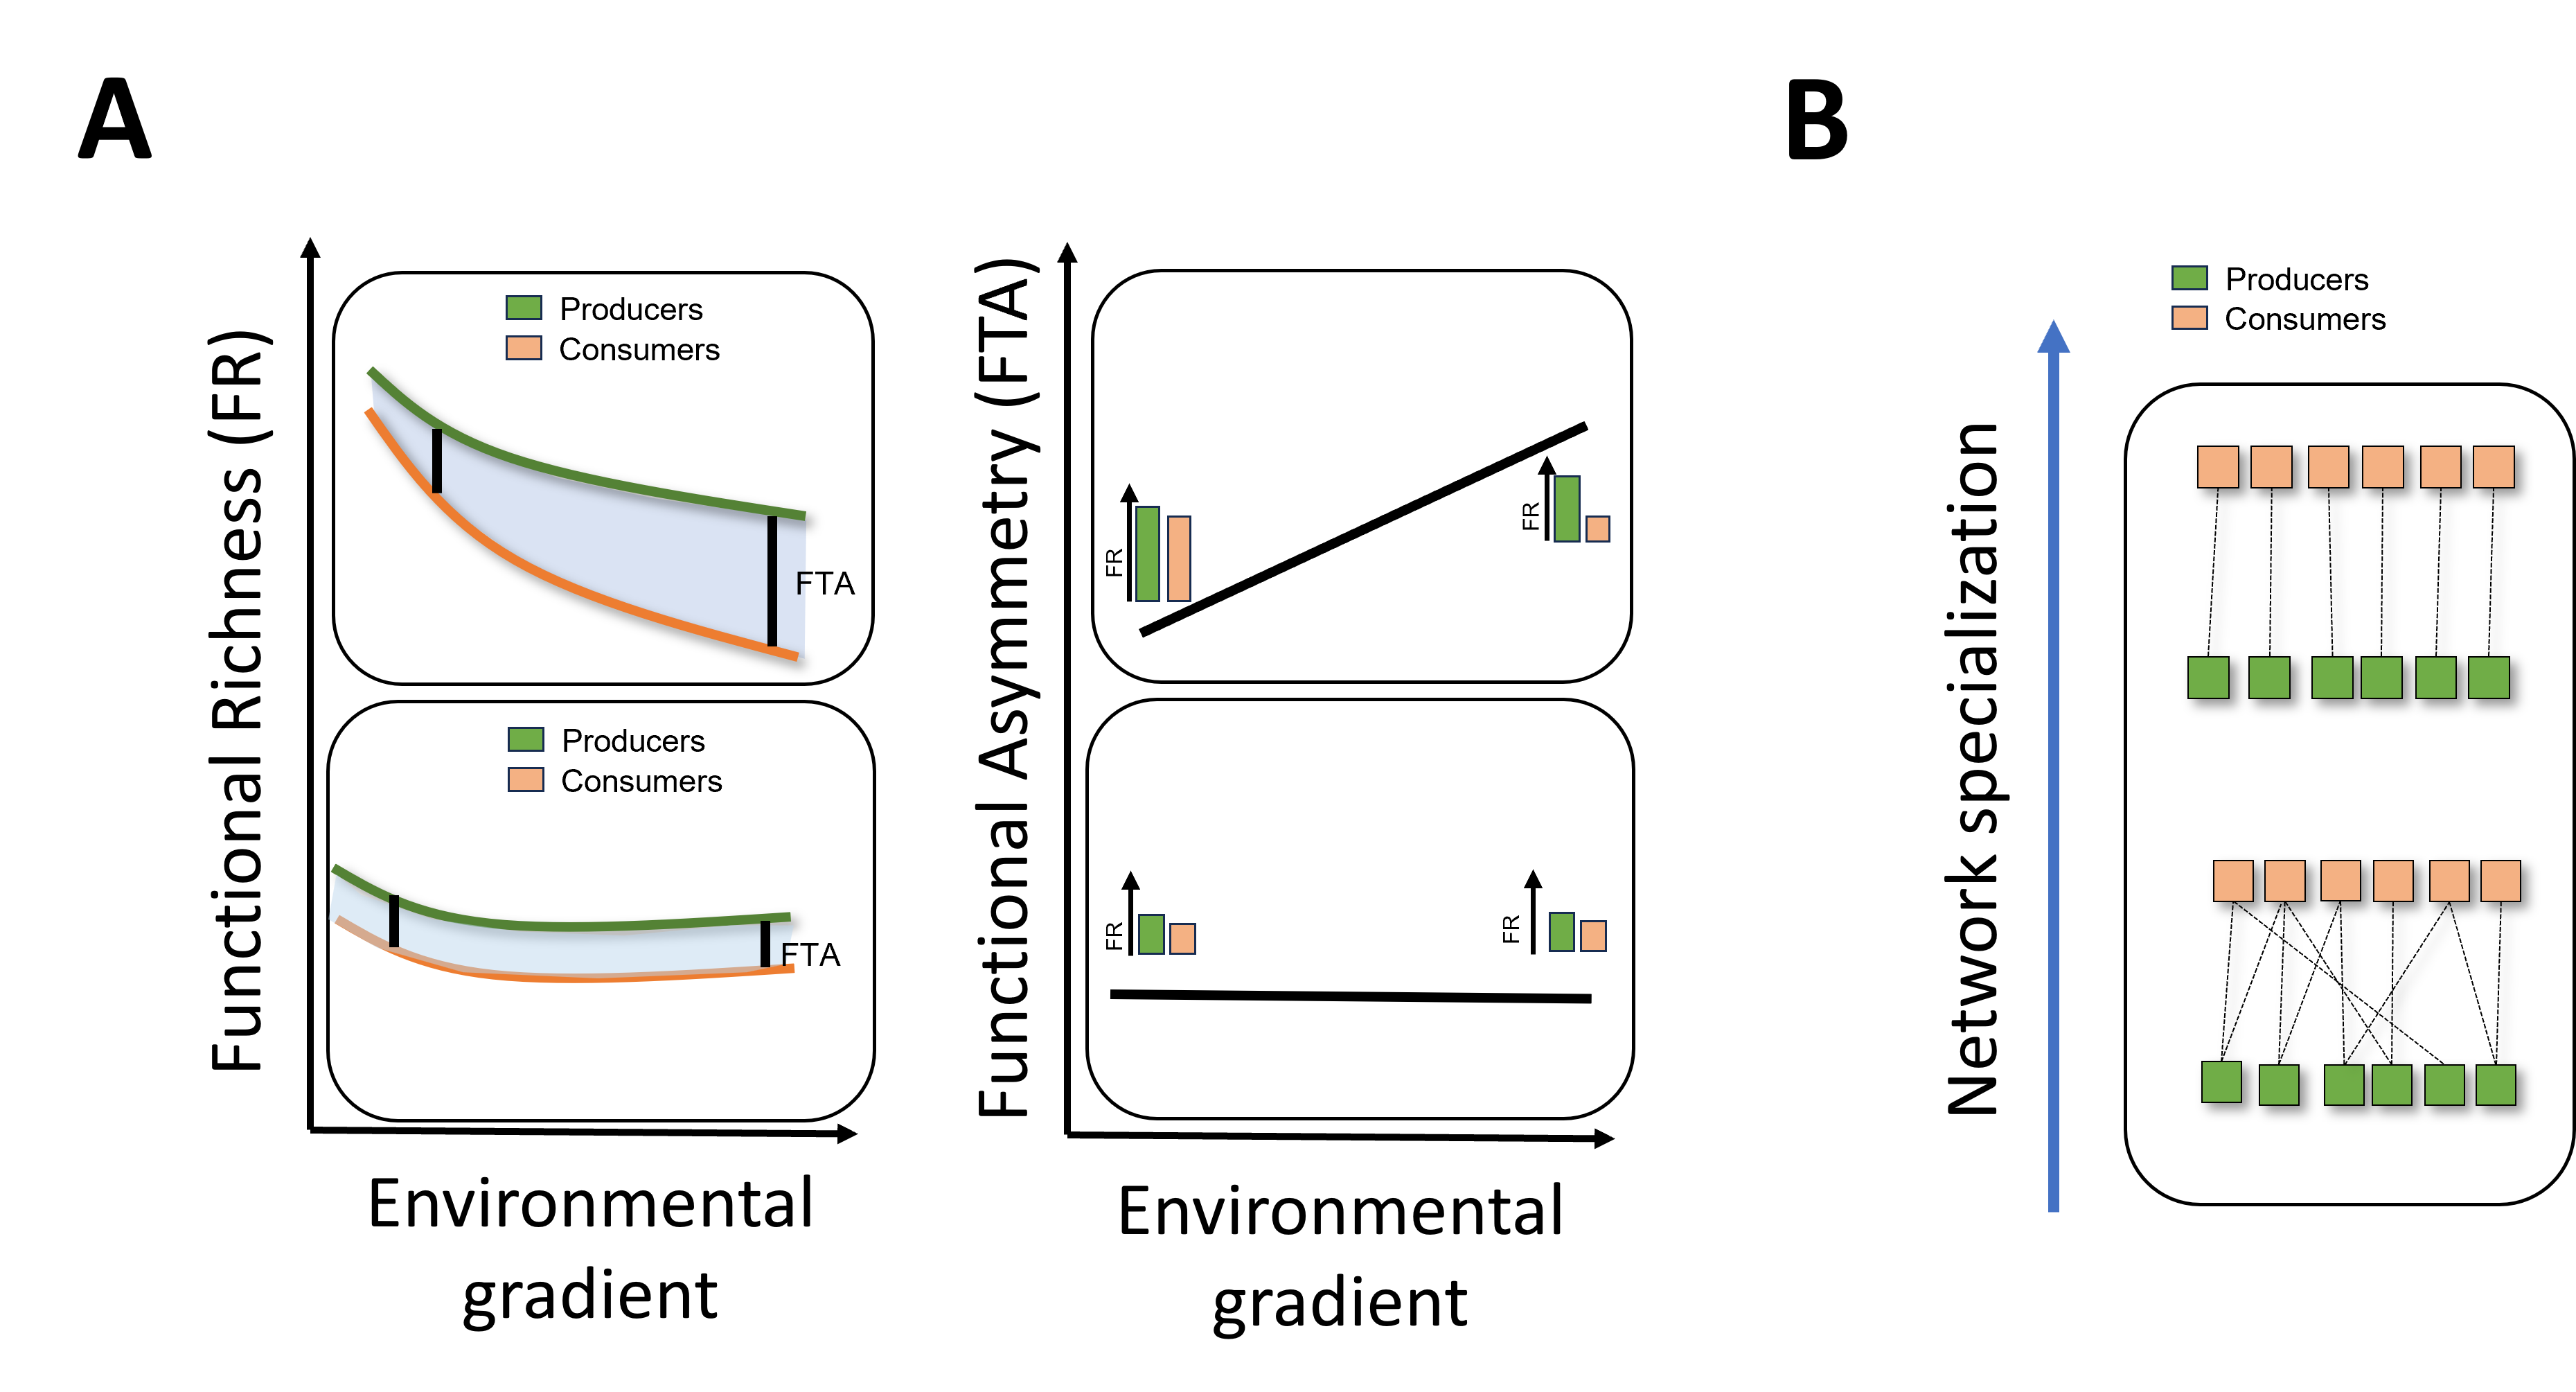
\includegraphics{Main_figures/00_Figure1.png}

}

\caption{Figure 1: This conceptual model illustrates the dynamic
relationship between functional diversity metrics---specifically
Functional Richness (FR) and Functional Trait Asymmetry (FTA)---and
environmental gradients within ecological networks. The left panel of
\textbf{Figure A} visualizes the variation in FR for producers (depicted
in green) and consumers (depicted in orange) along an environmental
gradient. As the environmental gradient intensifies (e.g., through
changes in temperature, precipitation, or habitat fragmentation), FR for
both producers and consumers generally declines. However, this decline
can occur at different rates, leading to two scenarios: (1)
\textbf{Differential Decline in FR}: If consumer FR declines more
sharply than producer FR, a substantial increase in Functional Trait
Asymmetry (FTA) occurs. (2) \textbf{Parallel Decline in FR}:
Alternatively, if both producer and consumer FRs decline at a similar
rate, FTA remains relatively constant along the gradient. This scenario
indicates a balanced impact of environmental changes across trophic
levels, preserving the relative functional relationship between
producers and consumers. \textbf{Figure B} shifts focus to the
implications of changing FTA on network specialization---a measure of
how distinct or generalized interactions are between producers and
consumers within ecological networks. \textbf{Higher Specialization}:
This scenario, shown on the left side of the gradient, involves more
distinct producer-consumer interactions, where specific consumer species
interact with particular producer species. This high specialization
often correlates with low FTA, where the functional traits between
interacting species are closely aligned. \textbf{Lower Specialization}:
As environmental stress increases, leading to a higher FTA, the network
may shift towards lower specialization. In this state, interactions
become more generalized, with consumers utilizing a broader range of
producers due to the loss of specific functional traits.}

\end{figure}%

\section{Methods}\label{methods}

In this study, we investigated the variation of functional trophic
asymmetry and network specialization along climatic gradients by
gathering species-level information on traits, interactions, and
distributions from literature, museum specimens, and field collections.
The collected data were then processed to create synthetic networks
across gridded regions of the Neotropics and to calculate functional
trophic asymmetry and network specialization variables, followed by
using climate data to explain the variation in these variables across
the Neotropics (Figure S1).

\subsection{Study system}\label{study-system}

We focused on multitrophic communities of Neotropical palms and their
mutualistic, seed dispersing, mammalian frugivores. Palms
(Plantae:Arecaceae), being a keystone plant family in tropical regions
(Kissling et al., 2012; Onstein et al., 2017), provide fruit resources
to a wide variety of vertebrate frugivores, including birds and mammals
(Muñoz et al., 2019; Zona \& Henderson, 1989). Frugivore mammals
(Animalia:Mammalia) are among the most important palm-seed dispersers,
particularly over long distances. Most frugivore mammals feeding on
palms are seed eaters and pulp eaters, dispersing palm seeds mostly via
ectozoochorus dispersal (Messeder et al., 2020). Importantly,
frugivory-related traits have notably underlain palm diversification and
played a key role in the evolution of palm traits (Onstein et al., 2014,
2017)

\subsection{Data collection}\label{data-collection}

\subsubsection{Species level geographic distribution
data}\label{species-level-geographic-distribution-data}

We obtained binary species distribution data (present/absent) on palms
from the geographic range maps of (Bjorholm et al., 2005) and on mammals
from the IUCN (International Union for the Conservation of Nature) data
portal. To generate local gridded multitrophic species assemblages
across the Neotropics, we intersected the species-level range maps with
a spatial grid where each grid cell represented every 1 by 1 degree
latitude and longitude change along the extent of the entire Neotropics.
We then listed all palm and mammal frugivore species co-occurring in
each grid-cell as our grid-cell level multitrophic assemblage.

\subsubsection{Species level trait data}\label{species-level-trait-data}

We collected species-level multitrophic trait data related to the
physiological tolerance of palms and frugivorous mammals to the abiotic
environment and to their mutualistic interactions. For palms, we
extracted data from the PalmTraits 1.0 dataset (Kissling et al., 2019).
We collected data on growth form, maximum stem height, and average fruit
length. For frugivorous mammals, we obtained trait data from the
EltonTraits 1.0 database (Wilman et al., 2014). We selected data on body
mass, diet, and daily activities. Diet data from the EltonTraits 1.0
database is coded as percentage use distribution across ten diet
categories. We excluded from our analysis species without fruit in their
diet. Activity was coded as a dummy variable with three categories
(Diurnal, Crepuscular, Nocturnal). Finally, body mass was coded as a
numerical variable in kg. We excluded bats from the analysis as almost
no Neotropical bat species is feeding on palm fruits (Messeder et al.,
2020). In total, we subset from this dataset the species with available
distribution range map, that is 494 palm species and 737 mammal
frugivores.

\subsubsection{Pairwise species level interaction
data}\label{pairwise-species-level-interaction-data}

We used data on seed dispersal interactions between palms and mammals
for the Neotropics, originating from recollections of seed dispersal
records found in the published literature and interaction records are
recorded at the species level (Muñoz et al., 2019). Each pairwise
species interaction record reflects where an article mentions the fruit
or the seed of a palm being dispersed, carried or defecated by a
frugivorous mammal. Interaction records collected in this database were
previously vetted to reflect effective seed dispersal interactions,
while avoiding those that reflect mere seed consumption (vetting
criteria found in: (Muñoz et al., 2019)). In total, we gathered a total
of 581 interaction records between 69 palms and 111 frugivore mammals.

\subsubsection{Grid-cell level environmental
data}\label{grid-cell-level-environmental-data}

We used bioclimatic variables from WorldClim (Fick \& Hijmans, 2017) to
represent large-scale spatial and temporal variation of climate in the
Neotropics. Specifically, we used mean annual temperature (BIO01), total
annual precipitation (BIO12), temperature seasonality (BIO04) and
precipitation seasonality (BIO15). Using a moving window, we compute
simple averages for every set of bioclimatic records at each grid cell,
thereby re-scaling the spatial resolution of bioclimatic variables to 1
by 1 degree grid resolution from their original resolution (1 by 1 km2)
to match the spatial resolution of our grid cell species-level data.

\subsubsection{Continental level biogeographical
data}\label{continental-level-biogeographical-data}

The Neotropics is a region with a rich evolutionary history which
significantly influenced patterns of species colonization and extinction
across neotropical plant and animal species (Antonelli \& Sanmartı́n,
2011; Whiteman-Jennings, 2015) . The biogeographic regionalization
patterns of (Morrone, 2014) distinguish seven major biogeographic
regions (i.e., biogeographic dominions), we use them to delineate the
spatial extent of species pools when simulating network assembly
processes.

\subsection{Statistical analyses}\label{statistical-analyses}

\subsubsection{A probabilistic continental
metaweb}\label{a-probabilistic-continental-metaweb}

Here, we fitted latent variable models that vary in their assumptions to
estimate interaction probabilities from observed binary data on species
interactions. Specifically: the stochastic block model (SBM), the
connectance model, the trait-matching model, and the matching-centrality
model (Terry \& Lewis, 2020). The SBM assumes that ecological networks
are modular, with species interacting more within their groups, and
outputs an two incidence matrix for palm and mammal species group
affiliations, and a squared matrix (Theta matrix) for interaction
probabilities. The connectance model posits that interactions of
specialist species are subsets of those of generalist species,
optimizing connectivity scores to recreate observed network patterns.
The trait-matching model assumes non-random species interactions
determined by trait differences, optimizing parameters along
latent-trait axes. The matching-centrality model combines connectivity
scores and latent-trait axes (Terry \& Lewis, 2020). We fitted these
models to our available interaction data and selected the model that
best predicted the observed continental pattern of seed dispersal
interactions. Using Youden's J as a metric that balanced model
sensitivity and specificity (Poisot, 2023), we find that SBM was the
best supported model (Figure S2 A-C). Additional details about the model
assumptions are explained in \emph{\textbf{Supplementary Text S1}.}

\subsubsection{Downscaling the continental metaweb to generate grid-cell
level
networks}\label{downscaling-the-continental-metaweb-to-generate-grid-cell-level-networks}

The digitally availability of primary biodiversity data on palms and
their mammalian frugivores was imbalanced, with well covered data in
terms of distribution ranges, followed by well covered data on species
traits, to a limited number of interaction records. Therefore, to
downscale our initial metaweb to include interactions between between
every potentially co-occurring palms and mammal frugivore at every
gridcell of the Neotropics, we use a two fold approach. First, we
employed multinomial logistic regression models that aimed to predict
the species level SBM model results~(i.e.~group affiliations) from
species-level trait data. We justify the choice of multinomial logistic
regression models as these can handle the prediction of non-binary
outcomes, that is in our case, the labeling of SBM groupings per
species. We fitted separate multinomial models for palms and mammal
frugivores using a label backpropagation algorithm and a neural network
engine, with 75\% of the data allocated for training and the 25\%
remaining for testing. We used neural networks because they are useful
when dealing with multicollinearity, as they can learn complex and
non-linear relationships and interactions among predictor variables.
This allowed us to separate the relative importance of distinct matching
traits on SBM group affiliations. We extracted variable importance
scores based on the combinations of the absolute values of the best fit
model weights (Gevrey et al., 2003). Second, we considered as local
pairwise species interaction probabilities as the product of the values
from the Theta matrix from the SBM model that represent the latent
interaction probabilities between species pairs within and between
groups multiplied by their probability of co-occurrence (POC) in a
gridcell. To represent species' co-occurrence probabilities, we used the
reciprocal distance between the centroids of species pair ranges within
the grid-cell, divided by the sum of its range areas within the
grid-cell. This implied that within each grid cell, species with closer
range centroids and larger cumulative areas are more likely to co-occur
and interact. This approach allowed us to recreate synthetic
probabilistic plant-mammal frugivore networks for each grid-cell across
the Neotropics, while accounting for the heterogeneity of species ranges
within each grid.

\subsubsection{Measuring Functional Trophic Asymmetry (FTA) and Network
Specialization
(H2')}\label{measuring-functional-trophic-asymmetry-fta-and-network-specialization-h2}

We computed Functional Trophic Asymmetry (FTA) from the results of the
SBM model fit. Specifically, from the matrices representing the
incidence of palm or mammal frugivore species in one of the SBM
groupings. Thus, as our measure of functional richness, we calculated
the number of species of each taxon across SBM groups per grid. Because
we had differences in the total number of palm and mammal species across
grids, we normalized species counts within gridcells. We then computed
the absolute difference between trophic levels to obtain a measure of
FTA for each combination of SBM groups. Because we had the potential for
each palms and mammals species at each grid to become affiliated to any
of 7 SBM groups, and to interact with any species of the opposite
trophic level within and between groups, we obtained a total of 49
independent FTA measures for each gridcell, one for each palm-mammal
group combination.

We measured network specialization at each grid cell using the metric
H2'. H2' is a network-level index that describes the degree of
specialization of interactions between species (Blüthgen et al., 2007).
High values indicate networks that are more specialized, meaning that
specialist species from one trophic level interact with specialist
species from the opposite trophic level. Low H2' values indicate
networks among generalists, meaning that there is a low specificity of
interactions between species across trophic levels. Because inferred
networks varied in their network size (i.e., number of unique
interactions between palms and mammals), we rarefied the computation of
H2'to networks of the same absolute size per gridcell, resampling
networks to the same number of pairwise interactions (100) at each
grid-cell 999 times (Terry \& Lewis, 2020). We selected the median of
this H2' distribution as our gridcell level measure of network
specialization.

We assessed the deviance of `observed' FTA and H2' from null models that
simulated stochastic community assembly processes (Dormann et al.,
2009). We created these null models by constructing networks of
interactions between a randomized set of palms and mammals for each
gridcell and computing expected values of FTA and H2'. To do this for a
given gridcell, we identified their biogeographic domain (from (Morrone,
2014)) and randomly sampled 10 palm and mammal species, ensuring each
species is selected only once. To this subsampled species set, we used
the same procedures to calculate FTA and H2' and replicated the process
999 independent times to obtain a distribution of expected FTA and H2'
values. Finally, we computed the deviance between observed and expected
values with Z-scores.

\subsubsection{Assessing the influence of climate in Functional Trophic
Asymmetry}\label{assessing-the-influence-of-climate-in-functional-trophic-asymmetry}

We fitted linear regression models to investigate the influence of
climate to Functional Trophic Asymmetry. We used FTA z-scores as
response variables and the four climatic predictor variables: Mean
Annual Temperature (Temp), Total Annual Precipitation (Prec),
Temperature Seasonality (TS), and Precipitation Seasonality (PS) as
predictor variables. In addition, we included the identity of the SBM
palm-mammal group combination as an interaction term. Prior to fitting
the models, we scale-transformed the climatic variables such that they
all share the same mean but only differ in their standard deviation.

\subsubsection{Assessing the influence of Functional Trophic Asymmetry
in Network
Specialization}\label{assessing-the-influence-of-functional-trophic-asymmetry-in-network-specialization}

We fitted linear regression models to investigate the effects of
Functional Trophic Asymmetry in Network specialization. We used the
average (mean) and standard deviation (sd) of FTA across all gridcells
and SBM combinations as our predictor variables. By including both as
predictors, the model accounts for not only the overall asymmetry but
also its distribution among SBM groupings. We used the rarefied gridcell
records of H2' as our response variable. To asses model significance, we
compared the estimates of this model to a distribution of expected model
coefficients from fitting the same linear model for each of the null
network assembly replicates.

\section{Results}\label{results}

\subsection{The structure of mutualistic networks between palms and
their mammalian frugivores across the
Neotropics}\label{the-structure-of-mutualistic-networks-between-palms-and-their-mammalian-frugivores-across-the-neotropics}

The SBM model organized the continental set of palm and mammal species
into a matrix sorting species into seven SBM groups and an accompanying
matrix that quantified interaction probabilities between and within
groups. In our model, there was a 1.74 fold increase in the likelihood
of interactions between species within SBM groups rather than between
SBM groups (Figure 2A). For palms, important trait variables that
predicted SBM group affiliation were palm fruit length, maximum stem
height, and palm growth form (\emph{Acaulescent} or \emph{Erect})
(Figure S3-A). For mammals, important trait variables to predict species
group affiliations were mammal activity, the logarithm of the \emph{body
mass}, and percentage of frugivory on diet as predictor variables
(Figure S3-B). These analysis revealed that SBM group assortments
represent communities of palms (Figure S4) and mammal frugivores (Figure
S5) with unique trait combinations within the high-dimensional
multitrophic spectrum of interaction-relevant traits. Our approach to
downscale a continental metaweb was able to generate probabilistic
networks between palms and mammalian frugivores for 1,072 grid cells
acrosss the Neotropics. Each network had in average nine interaction
partners per species (sd = 5.62), 27 mammals per grid cell (sd = 14.97),
and 11 palms per grid cell (sd = 11.42).

\begin{figure}

{\centering 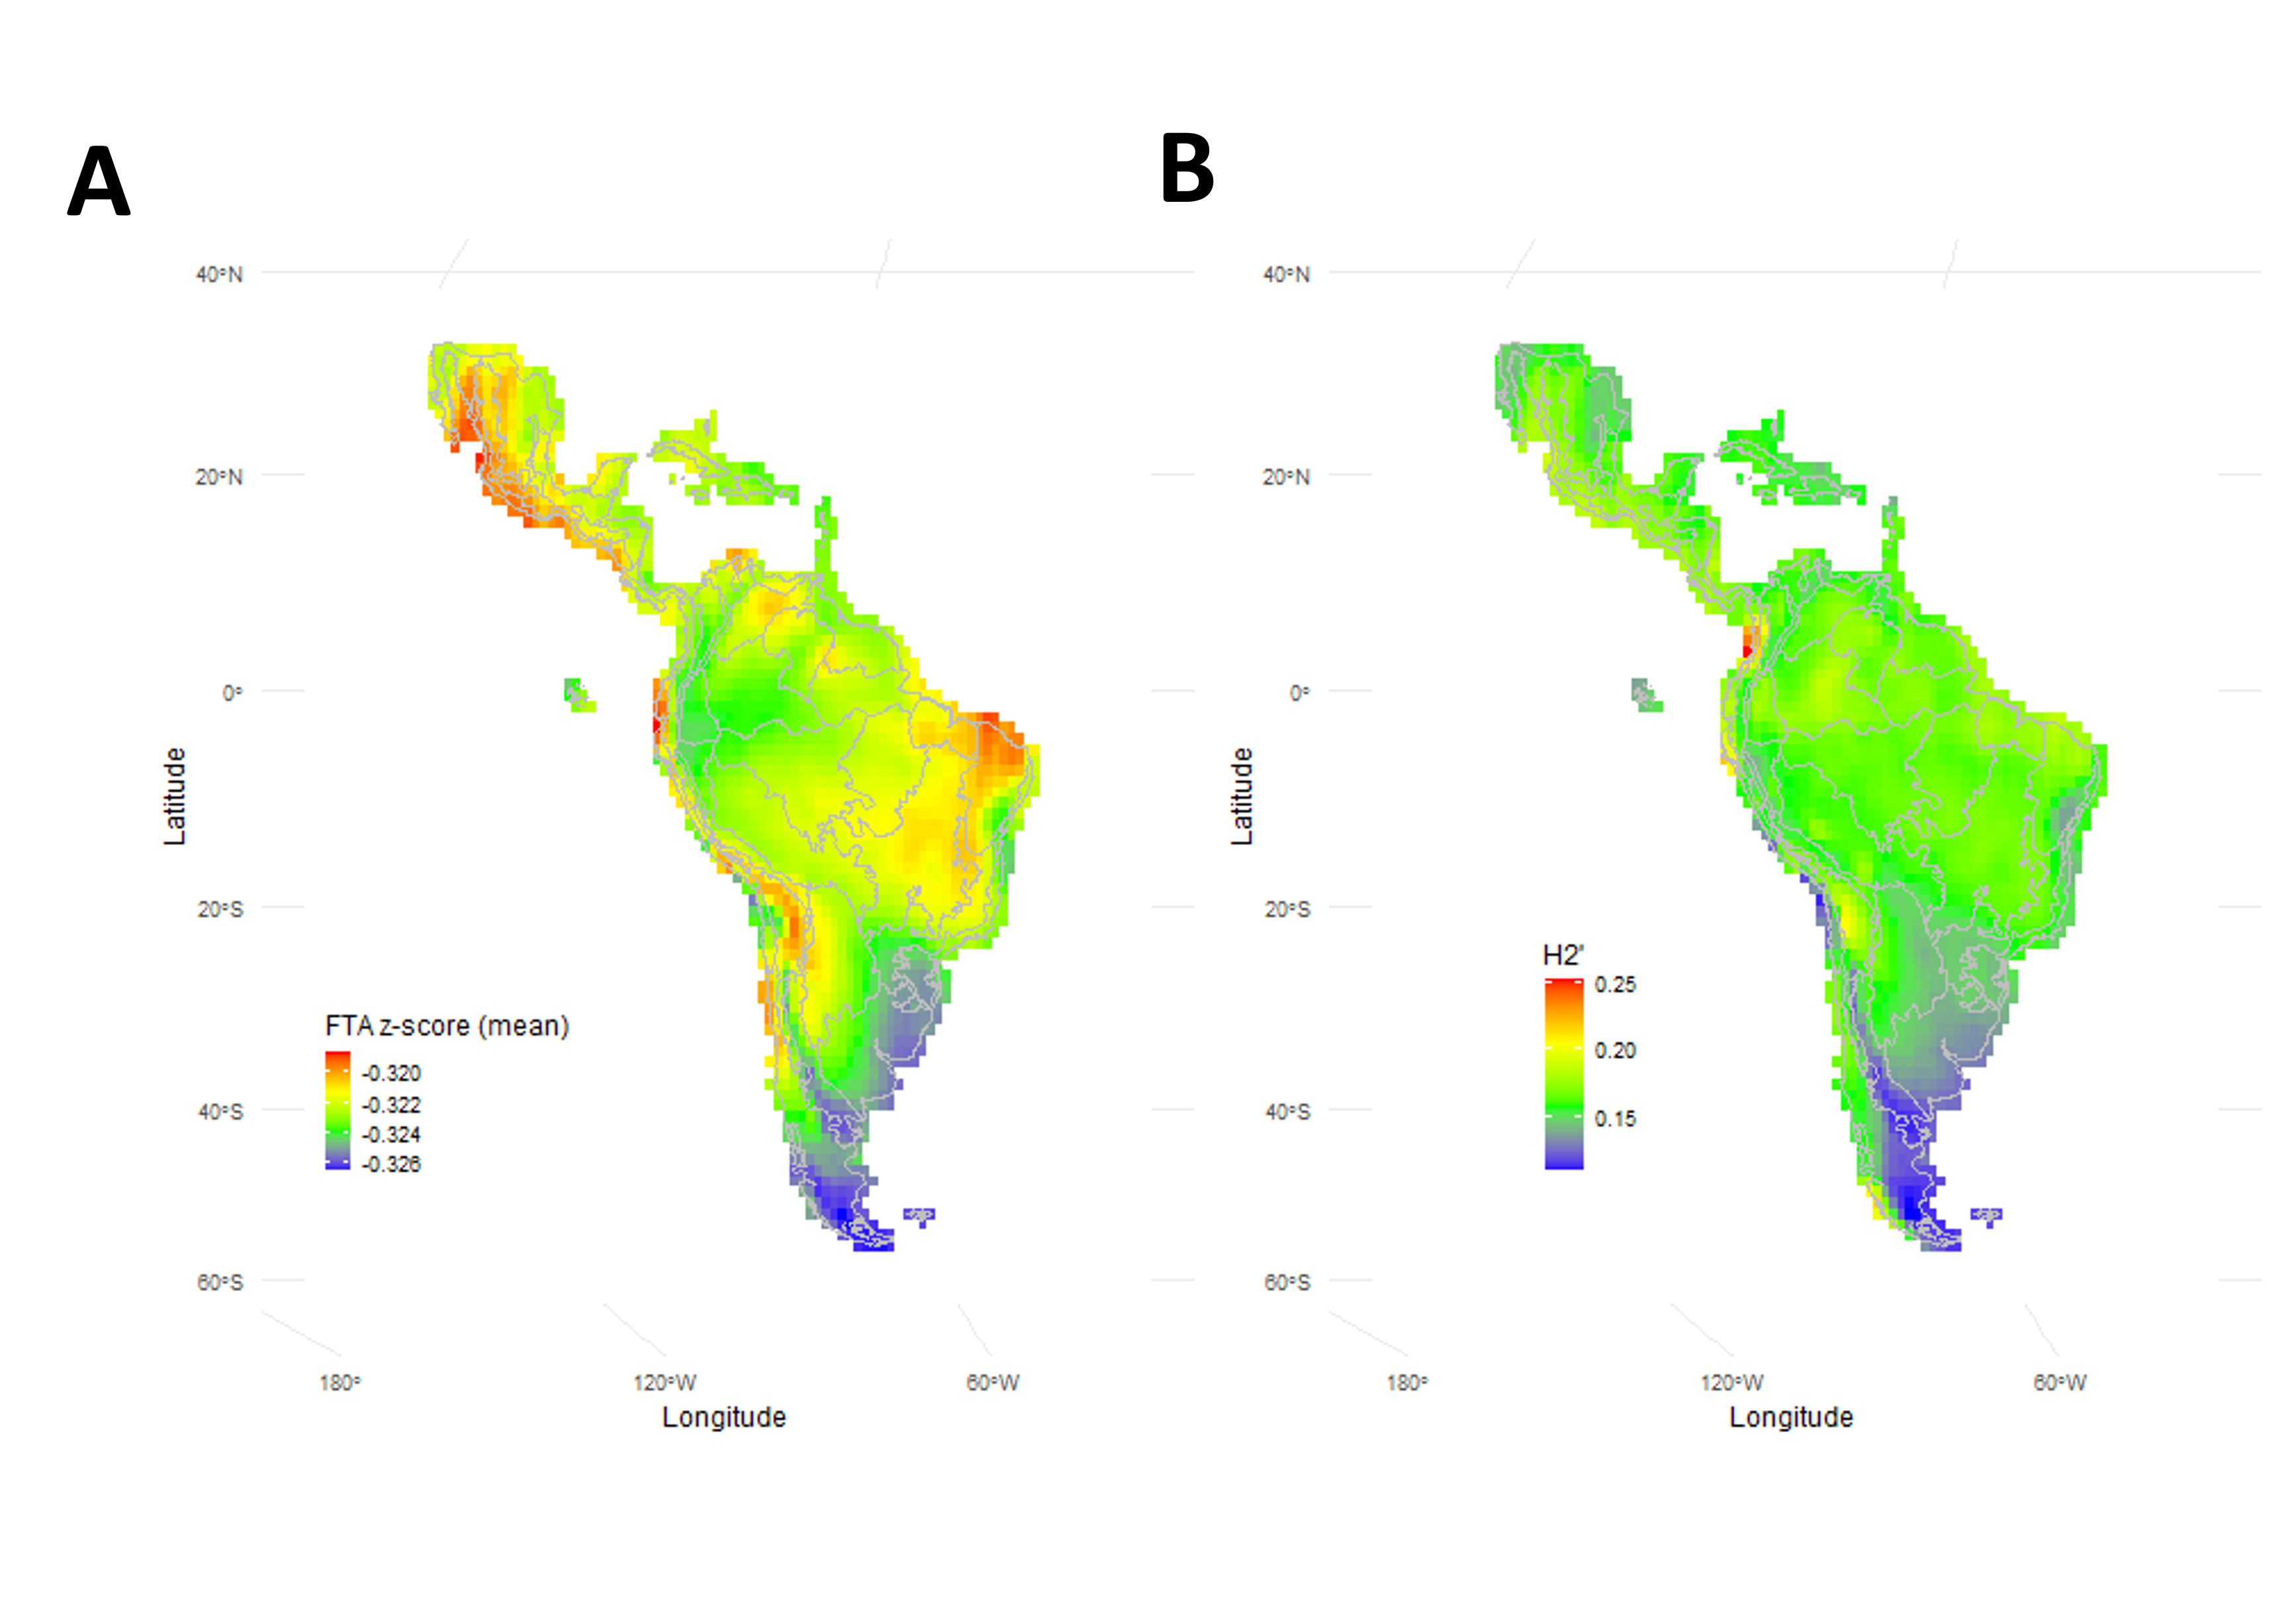
\includegraphics{Main_figures/00_network_maps.tif.png}

}

\caption{Figure 2: Spatial distribution of \textbf{(A)} FTA z-score
(mean) and \textbf{(B)} H2' network specialization index across the
Neotropics. Panel A depicts the geographic variation in the mean
z-scores of the Functional Trophic Asymmetry (FTA). Areas with higher
z-scores indicate greater asymmetry in the richness of interaction
relevant traits between trophic levels, whereas lower scores suggest
more balanced trait distributions. Panel B presents the spatial
distribution the degree of species specialization of interactions within
ecological networks. This panel reveals significant latitudinal
gradients, particularly marked in the Andes and the Southern Cone.}

\end{figure}%

\subsection{Differences in trait-climate relationships across trophic
levels lead to Functional Trophic
Asymmetry}\label{differences-in-trait-climate-relationships-across-trophic-levels-lead-to-functional-trophic-asymmetry}

FTA z-scores \hyperref[fig2]{(Figure 2B)} indicate that in average FTA
was less than the FTA expected from a null assembly model. Out of the 49
SBM group combinations, those with less than expected asymmetries are
generally between palms in groups 1, 2, and 5 and mammals in groups 6
and 3. Conversely, combinations with significantly greater than expected
asymmetries are generally found between palms in SBM groups 6 and 4 and
mammals in SBM groups 1, 2, and 5. FTA peaks in tropical and mountainous
regions while being lower in more temperate areas of the Neotropics, and
remains stable throughout tropical and humid regions (Figure 2A). The
results of our linear model shows significant differences in FTA among
SBM groups. In addition, it shows a relationship between the spatial
variation of climate and FTA. However, the significance and direction of
effects vary as a function of the SBM group combinations (Figure 3B,
Table 1). While the overall fixed model estimates do not show
significant effects of climatic variation in FTA across all SBM group
combinations {[}Temp (Mean annual temperature) ( 𝞫 =0.0051, p=0.859),
Prec (Total annual precipitation) ( 𝞫 =−0.0364 p=0.384), TS (Temperature
Seasonality) (𝞫 =−0.0180 p=0.746), and PS (Precipitation Seasonality) (𝞫
=−0.0507 p=0.250){]}; for specific group combinations, FTA is
significantly predicted by climate, particularly by changes in
Precipitation Seasonality (Figure S6). Approximately 59\% of the
variability in the FTA z-score is explained by the linear model with our
climate predictors as fixed effects and SBM group identity as
interaction terms (adjusted R-squared = 0.59).

On one hand, group combinations exhibiting a positive relationship
between FTA and precipitation seasonality are characterized by a
relatively stable functional richness of mammals across gradients of
precipitation seasonality, while the functional richness of palms
increases under these conditions (Figures S6, S7). A significant portion
of this pattern can be attributed to turnover within the palm community
of SBM group 6, which predominantly consists of small to medium-sized
drupes or berries. These palms, which belong to genera such as
\emph{Acrocomia}, \emph{Allagoptera}, and \emph{Astrocaryum} are
typically of tropical origin and display diverse growth forms, including
both erect and acaulescent. Conversely, group combinations showing a
negative association between FTA and precipitation seasonality are
primarily driven by patterns in the palm community of SBM group 5
(Figures S6, S7). In this scenario, while the functional richness of
mammals remains stable, the functional richness of these palms,
generally characterized by species with erect growth forms and large
fruits, increases in regions with low precipitation seasonality.

\begin{figure}

{\centering 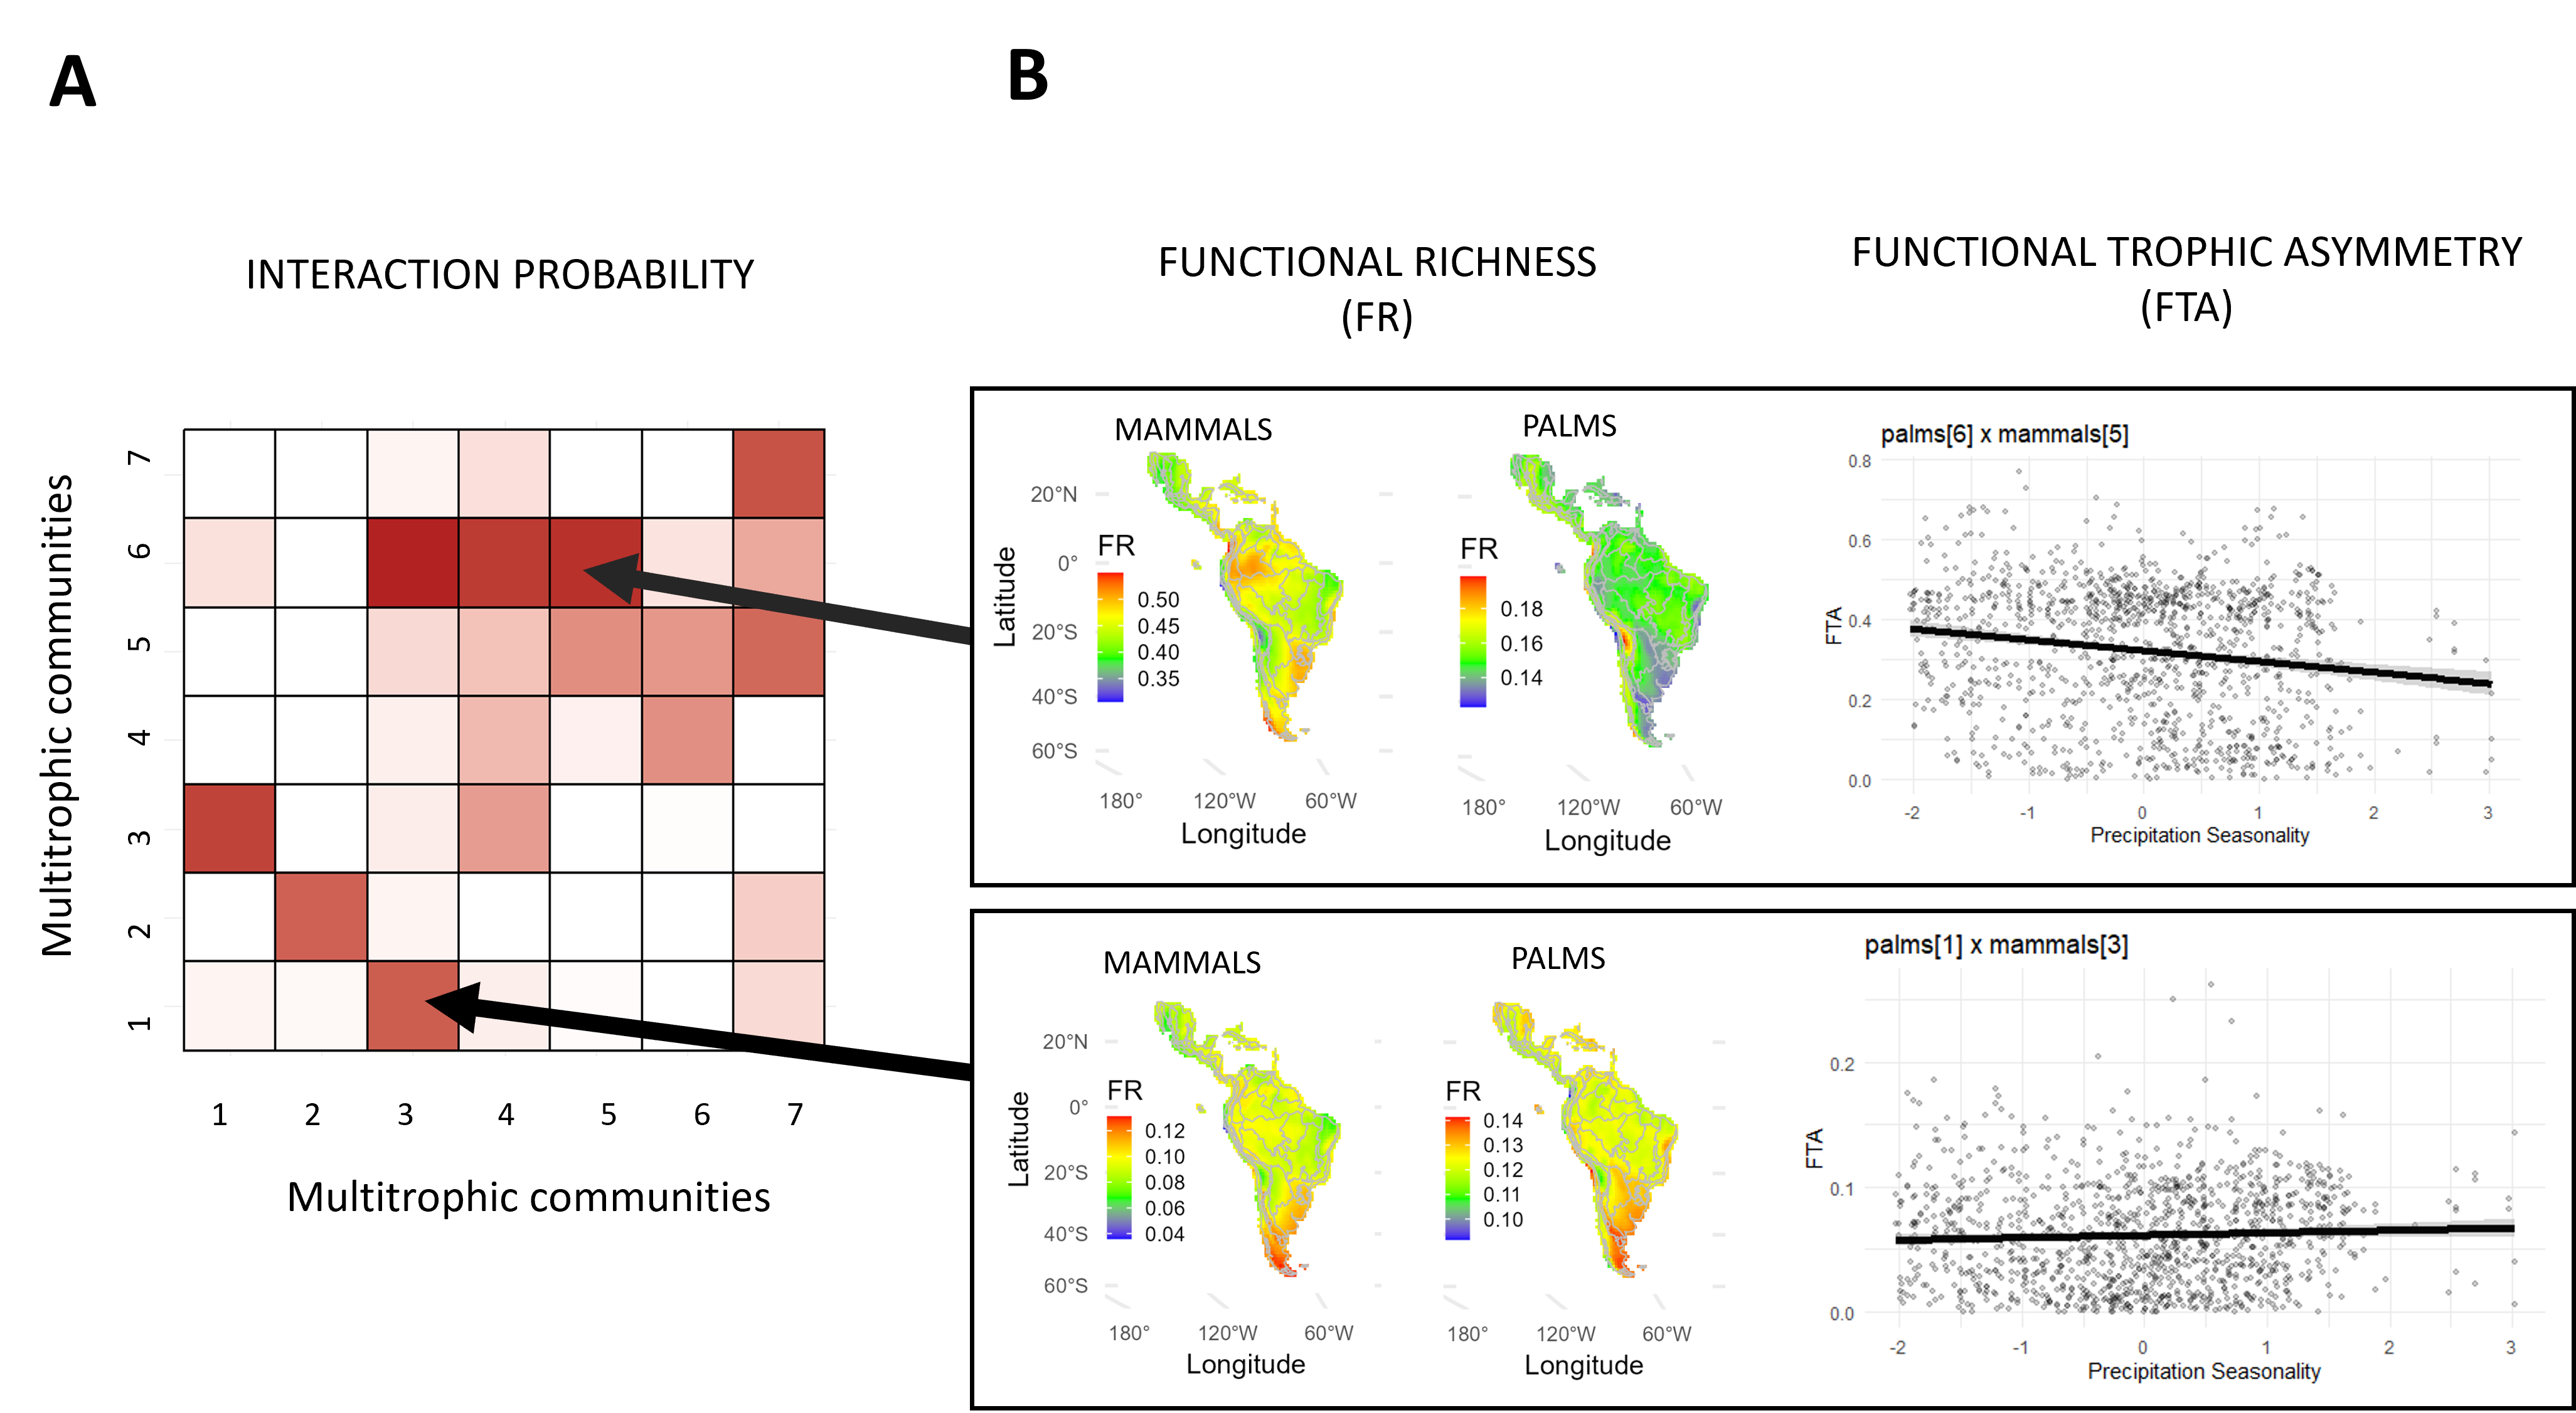
\includegraphics{Main_figures/00_network_fr.png}

}

\caption{Figure 3: \textbf{(A)} Heatmap depicting the interaction
probability among various multitrophic communities across different SBM
(Stochastic block model) groups. The intensity of red shading correlates
with the strength of these interactions, where darker shades signify
higher probabilities of interaction between species within or between
SBM groups. \textbf{(B)} The left panels present geographical maps
illustrating the distribution of FR for both mammals and palms,
identifying regions with distinct levels of functional diversity for a
given multitrophic combination of species at one SBM group pair. The
right panels illustrate the significant relationship observed between
FTA and precipitation seasonality.}

\end{figure}%

\subsection{Functional Trophic Asymmetry increases Network
Specialization}\label{functional-trophic-asymmetry-increases-network-specialization}

We found overall, palm-mammalian frugivore networks had low
specialization, H2' ranged from 0.12 to 0.25. In addition, there was a
significant relationship between aggregated gridcell records of
Functional Trophic Asymmetry and H2' metric. Specifically, FTA z-scores
increased H2' by 3.28 units per mean unit increase across all SBM
groups. Additionally, the standard deviation of FTA z-scores decreased
H2' by 1.01 units per unit increase across all SBM groups (SD FTA).
While this linear model explained only around 8.7\% of the total spatial
variability in H2' (adjusted R-squared = 0.087), the results of our
simulations show that the intercept and slope estimates are
statistically significant from null assembly models (Figure S7).

\section{Discussion}\label{discussion}

By making use of digitally available primary biodiversity data at broad
scales, our approach provides novel insights into the assembly of
mutualistic networks. By identifying species clusters of palms and
mammals with similar interaction patterns, we offer a more nuanced
understanding of network assembly dynamics within these multitrophic
communities. The distribution of Functional Trophic Asymmetry (FTA)
across different climatic regions of the Neotropics underscores the
importance of contemporary climate change in shaping interaction niches
across species' distributional ranges, with precipitation seasonality
emerging as a key predictor of FTA for certain SBM palm and mammal group
combinations, where higher FTA increase overall network specialization.

The delineation of interactions into distinct groups indicates that, at
a continental scale, the network of seed dispersal interactions is
highly compartmentalized. This finding aligns with previous work
reporting significant modularity in palm seed dispersal interactions
across the Neotropical continent (Muñoz et al., 2019). In our study, we
extend this understanding by identifying palm growth form and mammal
foraging activity periods as key palm and animal traits driving this
broad scale modularity through changes in functional richness. Clusters
of similarly interacting species obtained from SBM models such as ours
have been shown to reflect spatio-temporal segregation of species
assemblages and the differentiation of interaction niches
(Durand-Bessart et al., 2023). The observed distribution of interaction
probabilities within and between SBM groups highlights multitrophic
assemblages being central to the entire metaweb, notably the palm and
mammal species in SBM groups 5 and 6, which are those with extensive
distributional ranges and more generalist diets. Conversely, it also
identifies peripheral groups, such as species in SBM groups 1-3, which
exhibit narrower interaction niches. These peripheral species
assemblages may correspond to those species with restricted ranges or
specialized diets. Indeed, SBM groups 5-6 include larger, nocturnal
mammals that feed on palms with varying fruit sizes and growth forms,
ranging from erect to acaulescent, whereas SBM groups 1-3 predominantly
consist of smaller, diurnal mammals that consume small fruits from erect
palms.

Our linear model highlights Precipitation Seasonality as a key factor
predicting the Functional Trophic Asymmetry (FTA) in key SBM groupings.
This suggests that spatial variation in interaction niches emerges from
the differences in the strength of environmental selection between
trophic levels. Such uneven pressures result in multitrophic assemblages
where not all co-occurring trait combinations align optimally with the
global preferences between species interaction partners, thus
contributing to promote structural diversity in seed dispersal networks
across Neotropical sites. For example in SBM groups 1-3, mammalian
frugivores, which can exhibit a broad tolerance for varying levels of
precipitation seasonality, may predominantly consume small-fruited palms
in regions with high precipitation seasonality. This is likely because
palms with smaller fruits are better adapted to thrive under conditions
of variable water availability. Consequently, increased aridity
(e.g.~due to climate change) is expected to result in increased FTA,
driven by the restricted functional richness of available resources for
consumers. In SBM groups 5-6, palms with larger fruit sizes and
predominantly erect growth forms consumed by large sized frugivores
might reflect adaptations to attract high quality animal seed disperses
in environments where consistent water availability promotes higher
habitat complexity and plant competition. Consequently, increased
aridity is expected to result in increased FTA, but this time driven by
the restricted functional richness of available consumers relative to
producers. In both cases, FTA imposes limits over trait matching between
partners of distinct trophic levels and the partitioning of interaction
niches within species of the same trophic level.

The a low degree of specialization observed for palm-mammal frugivore
seed dispersal networks is not entirely unexpected given the historical
ecological shifts that these species have experienced in the Neotropics.
Unlike other major tropical regions, such as the Afrotropics and
South-East Asia, the Neotropics had significant post-Pleistocene
extinctions, which heavily altered mammalian communities. These
extinctions, which impacted disproportionately to mammal megafauna,
likely exacerbate competition and extinction rates among their
large-fruited palm partners, particularly in those regions with high
mammal diversity and endemism. (Webb, 2006; \textbf{whiteman2015?}) into
Concurrently, the radiation of small-fruited palm taxa (Onstein et al.,
2014, 2017) further contributed to the decoupling of trait diversity
between palms and mammals and the re-structuring of seed dispersal
networks across trophic levels in the Neotropics. Without this trait
decoupling due the co-evolutionary dynamics between palms and mammal
frugivores may have remained unaltered, fostering otherwise more
specialized networks.

The positive estimate for mean FTA suggests a strong positive influence
of FTA on H2', thus promoting network specialization. In contrast, the
negative estimate for FTA standard deviation (SD) indicates that a large
variation in FTA within SBM group combinations significantly reduces
H2', implying more generalist interactions. This suggest, that while
overall higher FTA promotes network specialization, an inconsistent FTA
across SBM groups can disrupt this pattern, making network structure
less predictable from multitrophic trait patterns. Previous research in
insular regions where trophic communities are often subject to
asymmetric filtering strengths have shown that the specialization of
mutualistic networks can indeed be resilient to shifts in the degree of
ecological filters between trophic levels. Particularly, if the networks
are well supported by generalist species (Schleuning et al., 2012 ;
Schleuning et al., 2016). It is therefore critical to consider changes
in the underlying network structure when evaluating potential effects
that climate-driven species or species trait losses have in ecosystem
function Classen et al. (2020)

We validated the statistic significance of the model parameters through
null simulations of network assembly,. However, it is noteworthy that
our null models are limited to presence/absence permutations. Therefore,
the potential influence of varying species relative abundances across
sites was not considered in this study. It is well established that
population-density dependent effects can modify interaction
probabilities from trait matching and range co-occurrences (Donoso et
al., 2017; McFadden et al., 2022; Peña et al., 2023). Future studies
should aim to incorporate species abundance estimates when defining
interaction probabilities. However, despite ongoing efforts, such data
is not readily available for multiple species at different trophic
levels, and at broad spatial scales. Our results help elucidate
mechanisms that contribute towards a broader theory of multitrophic
community assembly. However, given the current limitation in obtaining
reliable species abundance data, we advise caution when utilizing our
data pipelines for making finer-scale spatial predictions of network
assembly and interaction diversity. Similarly, the use biogeographic
domains to delineate the species pools in the construction of our null
models respects ecological theory and considers both historical and
regional species pools (Carstensen et al., 2013; Cornell \& Harrison,
2014; McFadden et al., 2022). However, one critical assumption of this
approach is that species within each biogeographic dominion are all
equally likely to colonize a given community (Lessard et al., 2012)
While this assumption may simplify the computational complexity of our
algorithms, future work could penalize dispersal distances with
landscape level variables such as the slope terrain (Préau et al., 2022;
Schlägel et al., 2020). Finally, the clustering of interactions captured
by the SBM may be also capturing reveal relatively unexplored drivers of
interaction assembly, such as phylogenetic niche conservatism (Ackerly,
2003; Pyron et al., 2015; Wiens \& Graham, 2005), where closely related
species retain similar ecological traits over evolutionary time, and/or
the widespread extinctions of large mammals frugivores and the rapid
trait speciation of small fruited palms (Donoso et al., 2020; Lim et
al., 2020; Onstein et al., 2017) . Partitioning these aspects and their
relative influences in delineating SBM group assignments can be future
research avenues to better understand the underlying mechanisms behind
mutualistic interaction patterns in space and time.

Unraveling the complexity of network assembly processes across broad
spatial scales requires continous development and refining of
statistical workflows and biodiversity data pipelines that integrate
digitally available data from diverse sources (Kissling et al., 2012;
Thuiller et al., 2024). Continued field collection, their open-release,
and data standardization is crucial if we want to expand our capacity to
training models capable of predicting ecological network structures at a
global scale with a high degree of spatial and/or temporal
resolution(Poisot et al., 2016, 2021). While many of these modelling
approaches are in early development, their success hinges on the
availability and reliability of foundational data. We have demonstrated
that with sparse data across large scales, novel models can indeed be
developed. Filling global data gaps and leveling data completeness
across species ranges, traits, and interactions can certainly enhance
predictive accuracy. While our case study has a history of digitally
available natural history data on both palms and mammal frugivores, such
comprehensive datasets are not available for many other tropical clades.
We thus advocate for increased awareness, action, and funding for global
biodiversity programs that collect and digitize natural records, thus
enabling the continous development of large-scale spatially explicit
predictive models that inform about mechanisms of network assembly, and
their relationship to climate and ecosystem function.

\section{Tables}\label{tables}

Table 1: Linear regression analysis of the relationship between
Bioclimatic Predictors (Mean Annual Temperature, Total Annual
Precipitation, Precipitation Seasonality, Temperature Seasonality) and
Functional Trophic Asymmetry within SBM groups (p1m1 - p7m7).
Statistically significant effects (p\textless0.05) are marked with (*).
Beta correspond to the variable effect coefficient in the model and SE
correspond to the standard error.

\setlength{\LTpost}{0mm}
\begin{longtable*}{lcc}
\toprule
\textbf{Characteristic} & \textbf{Beta}\textsuperscript{\textit{1}} & \textbf{SE}\textsuperscript{\textit{2}} \\ 
\midrule\addlinespace[2.5pt]
\textbf{Mean Annual Temperature} & 0.01 & 0.029 \\ 
\textbf{SBM group} &  &  \\ 
    p1m1 & — & — \\ 
    p1m2 & -0.65*** & 0.035 \\ 
    p1m3 & -0.50*** & 0.035 \\ 
    p1m4 & 0.00 & 0.035 \\ 
    p1m5 & -1.5*** & 0.035 \\ 
    p1m6 & 0.57*** & 0.035 \\ 
    p1m7 & 0.00 & 0.035 \\ 
    p2m2 & 0.77*** & 0.035 \\ 
    p2m3 & 0.42*** & 0.035 \\ 
    p2m5 & -2.0*** & 0.035 \\ 
    p2m6 & 0.84*** & 0.035 \\ 
    p3m1 & -1.4*** & 0.035 \\ 
    p3m2 & -1.7*** & 0.035 \\ 
    p3m3 & -1.5*** & 0.035 \\ 
    p3m4 & -1.4*** & 0.035 \\ 
    p3m5 & -0.22*** & 0.035 \\ 
    p3m6 & -1.8*** & 0.035 \\ 
    p3m7 & -1.4*** & 0.035 \\ 
    p4m1 & 0.15*** & 0.035 \\ 
    p4m2 & -0.12*** & 0.035 \\ 
    p4m3 & -0.59*** & 0.035 \\ 
    p4m4 & 0.15*** & 0.035 \\ 
    p4m5 & -1.8*** & 0.035 \\ 
    p4m6 & 0.47*** & 0.035 \\ 
    p4m7 & 0.15*** & 0.035 \\ 
    p5m2 & 0.77*** & 0.035 \\ 
    p5m3 & 0.42*** & 0.035 \\ 
    p5m5 & -2.0*** & 0.035 \\ 
    p5m6 & 0.84*** & 0.035 \\ 
    p6m1 & 1.5*** & 0.035 \\ 
    p6m2 & 0.03 & 0.035 \\ 
    p6m3 & 0.02 & 0.035 \\ 
    p6m4 & 1.5*** & 0.035 \\ 
    p6m5 & -2.7*** & 0.035 \\ 
    p6m6 & -0.01 & 0.035 \\ 
    p6m7 & 1.5*** & 0.035 \\ 
    p7m1 & 0.37*** & 0.035 \\ 
    p7m2 & -0.45*** & 0.035 \\ 
    p7m3 & -0.22*** & 0.035 \\ 
    p7m4 & 0.37*** & 0.035 \\ 
    p7m5 & -1.9*** & 0.035 \\ 
    p7m6 & 0.43*** & 0.035 \\ 
    p7m7 & 0.37*** & 0.035 \\ 
\textbf{Total Annual Precipitation} & -0.04 & 0.042 \\ 
\textbf{Temperature Seasonality} & -0.02 & 0.056 \\ 
\textbf{Precipitation Seasonality} & -0.05 & 0.044 \\ 
\textbf{Mean Annual Temperature * SBM group} &  &  \\ 
    Mean Annual Temperature * p1m2 & 0.01 & 0.040 \\ 
    Mean Annual Temperature * p1m3 & -0.01 & 0.040 \\ 
    Mean Annual Temperature * p1m4 & 0.00 & 0.040 \\ 
    Mean Annual Temperature * p1m5 & -0.01 & 0.040 \\ 
    Mean Annual Temperature * p1m6 & 0.04 & 0.040 \\ 
    Mean Annual Temperature * p1m7 & 0.00 & 0.040 \\ 
    Mean Annual Temperature * p2m2 & 0.02 & 0.040 \\ 
    Mean Annual Temperature * p2m3 & -0.06 & 0.040 \\ 
    Mean Annual Temperature * p2m5 & -0.01 & 0.040 \\ 
    Mean Annual Temperature * p2m6 & 0.02 & 0.040 \\ 
    Mean Annual Temperature * p3m1 & 0.05 & 0.040 \\ 
    Mean Annual Temperature * p3m2 & 0.04 & 0.040 \\ 
    Mean Annual Temperature * p3m3 & 0.06 & 0.040 \\ 
    Mean Annual Temperature * p3m4 & 0.05 & 0.040 \\ 
    Mean Annual Temperature * p3m5 & 0.05 & 0.040 \\ 
    Mean Annual Temperature * p3m6 & 0.06 & 0.040 \\ 
    Mean Annual Temperature * p3m7 & 0.05 & 0.040 \\ 
    Mean Annual Temperature * p4m1 & -0.05 & 0.040 \\ 
    Mean Annual Temperature * p4m2 & 0.08 & 0.040 \\ 
    Mean Annual Temperature * p4m3 & 0.00 & 0.040 \\ 
    Mean Annual Temperature * p4m4 & -0.05 & 0.040 \\ 
    Mean Annual Temperature * p4m5 & 0.01 & 0.040 \\ 
    Mean Annual Temperature * p4m6 & 0.05 & 0.040 \\ 
    Mean Annual Temperature * p4m7 & -0.05 & 0.040 \\ 
    Mean Annual Temperature * p5m2 & 0.02 & 0.040 \\ 
    Mean Annual Temperature * p5m3 & -0.06 & 0.040 \\ 
    Mean Annual Temperature * p5m5 & -0.01 & 0.040 \\ 
    Mean Annual Temperature * p5m6 & 0.02 & 0.040 \\ 
    Mean Annual Temperature * p6m1 & -0.05 & 0.040 \\ 
    Mean Annual Temperature * p6m2 & 0.06 & 0.040 \\ 
    Mean Annual Temperature * p6m3 & 0.03 & 0.040 \\ 
    Mean Annual Temperature * p6m4 & -0.05 & 0.040 \\ 
    Mean Annual Temperature * p6m5 & 0.01 & 0.040 \\ 
    Mean Annual Temperature * p6m6 & 0.05 & 0.040 \\ 
    Mean Annual Temperature * p6m7 & -0.05 & 0.040 \\ 
    Mean Annual Temperature * p7m1 & -0.03 & 0.040 \\ 
    Mean Annual Temperature * p7m2 & 0.08* & 0.040 \\ 
    Mean Annual Temperature * p7m3 & 0.01 & 0.040 \\ 
    Mean Annual Temperature * p7m4 & -0.03 & 0.040 \\ 
    Mean Annual Temperature * p7m5 & 0.00 & 0.040 \\ 
    Mean Annual Temperature * p7m6 & 0.04 & 0.040 \\ 
    Mean Annual Temperature * p7m7 & -0.03 & 0.040 \\ 
\textbf{SBM group * Total Annual Precipitation} &  &  \\ 
    p1m2 * Total Annual Precipitation & 0.01 & 0.059 \\ 
    p1m3 * Total Annual Precipitation & -0.05 & 0.059 \\ 
    p1m4 * Total Annual Precipitation & 0.00 & 0.059 \\ 
    p1m5 * Total Annual Precipitation & 0.10 & 0.059 \\ 
    p1m6 * Total Annual Precipitation & -0.08 & 0.059 \\ 
    p1m7 * Total Annual Precipitation & 0.00 & 0.059 \\ 
    p2m2 * Total Annual Precipitation & 0.04 & 0.059 \\ 
    p2m3 * Total Annual Precipitation & 0.10 & 0.059 \\ 
    p2m5 * Total Annual Precipitation & 0.10 & 0.059 \\ 
    p2m6 * Total Annual Precipitation & -0.06 & 0.059 \\ 
    p3m1 * Total Annual Precipitation & 0.04 & 0.059 \\ 
    p3m2 * Total Annual Precipitation & 0.04 & 0.059 \\ 
    p3m3 * Total Annual Precipitation & 0.02 & 0.059 \\ 
    p3m4 * Total Annual Precipitation & 0.04 & 0.059 \\ 
    p3m5 * Total Annual Precipitation & -0.11 & 0.059 \\ 
    p3m6 * Total Annual Precipitation & 0.05 & 0.059 \\ 
    p3m7 * Total Annual Precipitation & 0.04 & 0.059 \\ 
    p4m1 * Total Annual Precipitation & 0.03 & 0.059 \\ 
    p4m2 * Total Annual Precipitation & 0.00 & 0.059 \\ 
    p4m3 * Total Annual Precipitation & -0.06 & 0.059 \\ 
    p4m4 * Total Annual Precipitation & 0.03 & 0.059 \\ 
    p4m5 * Total Annual Precipitation & 0.10 & 0.059 \\ 
    p4m6 * Total Annual Precipitation & -0.06 & 0.059 \\ 
    p4m7 * Total Annual Precipitation & 0.03 & 0.059 \\ 
    p5m2 * Total Annual Precipitation & 0.04 & 0.059 \\ 
    p5m3 * Total Annual Precipitation & 0.10 & 0.059 \\ 
    p5m5 * Total Annual Precipitation & 0.10 & 0.059 \\ 
    p5m6 * Total Annual Precipitation & -0.06 & 0.059 \\ 
    p6m1 * Total Annual Precipitation & 0.11 & 0.059 \\ 
    p6m2 * Total Annual Precipitation & 0.02 & 0.059 \\ 
    p6m3 * Total Annual Precipitation & 0.07 & 0.059 \\ 
    p6m4 * Total Annual Precipitation & 0.11 & 0.059 \\ 
    p6m5 * Total Annual Precipitation & 0.06 & 0.059 \\ 
    p6m6 * Total Annual Precipitation & -0.10 & 0.059 \\ 
    p6m7 * Total Annual Precipitation & 0.11 & 0.059 \\ 
    p7m1 * Total Annual Precipitation & 0.02 & 0.059 \\ 
    p7m2 * Total Annual Precipitation & -0.03 & 0.059 \\ 
    p7m3 * Total Annual Precipitation & 0.06 & 0.059 \\ 
    p7m4 * Total Annual Precipitation & 0.02 & 0.059 \\ 
    p7m5 * Total Annual Precipitation & 0.10 & 0.059 \\ 
    p7m6 * Total Annual Precipitation & -0.05 & 0.059 \\ 
    p7m7 * Total Annual Precipitation & 0.02 & 0.059 \\ 
\textbf{SBM group * Temperature Seasonality} &  &  \\ 
    p1m2 * Temperature Seasonality & 0.01 & 0.079 \\ 
    p1m3 * Temperature Seasonality & 0.13 & 0.079 \\ 
    p1m4 * Temperature Seasonality & 0.00 & 0.079 \\ 
    p1m5 * Temperature Seasonality & 0.02 & 0.079 \\ 
    p1m6 * Temperature Seasonality & 0.16* & 0.079 \\ 
    p1m7 * Temperature Seasonality & 0.00 & 0.079 \\ 
    p2m2 * Temperature Seasonality & 0.01 & 0.079 \\ 
    p2m3 * Temperature Seasonality & -0.10 & 0.079 \\ 
    p2m5 * Temperature Seasonality & 0.01 & 0.079 \\ 
    p2m6 * Temperature Seasonality & 0.10 & 0.079 \\ 
    p3m1 * Temperature Seasonality & 0.03 & 0.079 \\ 
    p3m2 * Temperature Seasonality & 0.04 & 0.079 \\ 
    p3m3 * Temperature Seasonality & 0.08 & 0.079 \\ 
    p3m4 * Temperature Seasonality & 0.03 & 0.079 \\ 
    p3m5 * Temperature Seasonality & 0.17* & 0.079 \\ 
    p3m6 * Temperature Seasonality & 0.04 & 0.079 \\ 
    p3m7 * Temperature Seasonality & 0.03 & 0.079 \\ 
    p4m1 * Temperature Seasonality & -0.02 & 0.079 \\ 
    p4m2 * Temperature Seasonality & -0.02 & 0.079 \\ 
    p4m3 * Temperature Seasonality & 0.05 & 0.079 \\ 
    p4m4 * Temperature Seasonality & -0.02 & 0.079 \\ 
    p4m5 * Temperature Seasonality & 0.02 & 0.079 \\ 
    p4m6 * Temperature Seasonality & 0.12 & 0.079 \\ 
    p4m7 * Temperature Seasonality & -0.02 & 0.079 \\ 
    p5m2 * Temperature Seasonality & 0.01 & 0.079 \\ 
    p5m3 * Temperature Seasonality & -0.10 & 0.079 \\ 
    p5m5 * Temperature Seasonality & 0.01 & 0.079 \\ 
    p5m6 * Temperature Seasonality & 0.10 & 0.079 \\ 
    p6m1 * Temperature Seasonality & 0.09 & 0.079 \\ 
    p6m2 * Temperature Seasonality & 0.10 & 0.079 \\ 
    p6m3 * Temperature Seasonality & 0.14 & 0.079 \\ 
    p6m4 * Temperature Seasonality & 0.09 & 0.079 \\ 
    p6m5 * Temperature Seasonality & -0.04 & 0.079 \\ 
    p6m6 * Temperature Seasonality & 0.07 & 0.079 \\ 
    p6m7 * Temperature Seasonality & 0.09 & 0.079 \\ 
    p7m1 * Temperature Seasonality & -0.01 & 0.079 \\ 
    p7m2 * Temperature Seasonality & 0.06 & 0.079 \\ 
    p7m3 * Temperature Seasonality & 0.03 & 0.079 \\ 
    p7m4 * Temperature Seasonality & -0.01 & 0.079 \\ 
    p7m5 * Temperature Seasonality & 0.01 & 0.079 \\ 
    p7m6 * Temperature Seasonality & 0.11 & 0.079 \\ 
    p7m7 * Temperature Seasonality & -0.01 & 0.079 \\ 
\textbf{SBM group * Precipitation Seasonality} &  &  \\ 
    p1m2 * Precipitation Seasonality & -0.05 & 0.062 \\ 
    p1m3 * Precipitation Seasonality & 0.12* & 0.062 \\ 
    p1m4 * Precipitation Seasonality & 0.00 & 0.062 \\ 
    p1m5 * Precipitation Seasonality & -0.06 & 0.062 \\ 
    p1m6 * Precipitation Seasonality & 0.49*** & 0.062 \\ 
    p1m7 * Precipitation Seasonality & 0.00 & 0.062 \\ 
    p2m2 * Precipitation Seasonality & -0.09 & 0.062 \\ 
    p2m3 * Precipitation Seasonality & -0.09 & 0.062 \\ 
    p2m5 * Precipitation Seasonality & -0.14* & 0.062 \\ 
    p2m6 * Precipitation Seasonality & 0.39*** & 0.062 \\ 
    p3m1 * Precipitation Seasonality & 0.06 & 0.062 \\ 
    p3m2 * Precipitation Seasonality & 0.11 & 0.062 \\ 
    p3m3 * Precipitation Seasonality & 0.11 & 0.062 \\ 
    p3m4 * Precipitation Seasonality & 0.06 & 0.062 \\ 
    p3m5 * Precipitation Seasonality & 0.29*** & 0.062 \\ 
    p3m6 * Precipitation Seasonality & -0.04 & 0.062 \\ 
    p3m7 * Precipitation Seasonality & 0.06 & 0.062 \\ 
    p4m1 * Precipitation Seasonality & 0.00 & 0.062 \\ 
    p4m2 * Precipitation Seasonality & -0.09 & 0.062 \\ 
    p4m3 * Precipitation Seasonality & 0.06 & 0.062 \\ 
    p4m4 * Precipitation Seasonality & 0.00 & 0.062 \\ 
    p4m5 * Precipitation Seasonality & -0.09 & 0.062 \\ 
    p4m6 * Precipitation Seasonality & 0.43*** & 0.062 \\ 
    p4m7 * Precipitation Seasonality & 0.00 & 0.062 \\ 
    p5m2 * Precipitation Seasonality & -0.09 & 0.062 \\ 
    p5m3 * Precipitation Seasonality & -0.09 & 0.062 \\ 
    p5m5 * Precipitation Seasonality & -0.14* & 0.062 \\ 
    p5m6 * Precipitation Seasonality & 0.39*** & 0.062 \\ 
    p6m1 * Precipitation Seasonality & 0.22*** & 0.062 \\ 
    p6m2 * Precipitation Seasonality & 0.19** & 0.062 \\ 
    p6m3 * Precipitation Seasonality & 0.32*** & 0.062 \\ 
    p6m4 * Precipitation Seasonality & 0.22*** & 0.062 \\ 
    p6m5 * Precipitation Seasonality & -0.20** & 0.062 \\ 
    p6m6 * Precipitation Seasonality & 0.29*** & 0.062 \\ 
    p6m7 * Precipitation Seasonality & 0.22*** & 0.062 \\ 
    p7m1 * Precipitation Seasonality & 0.02 & 0.062 \\ 
    p7m2 * Precipitation Seasonality & -0.03 & 0.062 \\ 
    p7m3 * Precipitation Seasonality & 0.09 & 0.062 \\ 
    p7m4 * Precipitation Seasonality & 0.02 & 0.062 \\ 
    p7m5 * Precipitation Seasonality & -0.10 & 0.062 \\ 
    p7m6 * Precipitation Seasonality & 0.40*** & 0.062 \\ 
    p7m7 * Precipitation Seasonality & 0.02 & 0.062 \\ 
\bottomrule
\end{longtable*}
\begin{minipage}{\linewidth}
\textsuperscript{\textit{1}}*p\textless{}0.05; **p\textless{}0.01; ***p\textless{}0.001\\
\textsuperscript{\textit{2}}SE = Standard Error\\
\end{minipage}

\textsubscript{Source:
\href{https://fgabriel1891.github.io/quarto_template_rstudio/index.qmd.html}{Article
Notebook}}

Table 2: Linear regression analysis of the relationship between
Functional Trophic Asymmetry and Network Specialization. Statistically
significant effects (p\textless0.05) are marked with (*). Beta
correspond to the variable effect coefficient in the model and SE
correspond to the standard error.

\setlength{\LTpost}{0mm}
\begin{longtable*}{lcc}
\toprule
\textbf{Characteristic} & \textbf{Beta}\textsuperscript{\textit{1}} & \textbf{SE}\textsuperscript{\textit{2}} \\ 
\midrule\addlinespace[2.5pt]
\textbf{FTA (mean)} & 3.3*** & 0.327 \\ 
\textbf{FTA (sd)} & -1.0*** & 0.137 \\ 
\bottomrule
\end{longtable*}
\begin{minipage}{\linewidth}
\textsuperscript{\textit{1}}*p\textless{}0.05; **p\textless{}0.01; ***p\textless{}0.001\\
\textsuperscript{\textit{2}}SE = Standard Error\\
\end{minipage}

\textsubscript{Source:
\href{https://fgabriel1891.github.io/quarto_template_rstudio/index.qmd.html}{Article
Notebook}}

\section{References}\label{references}

\phantomsection\label{refs}
\begin{CSLReferences}{1}{0}
\vspace{1em}

\bibitem[\citeproctext]{ref-acevedo2020structure}
Acevedo-Quintero, J. F., Zamora-Abrego, J. G., \& Garcı́a, D. (2020).
From structure to function in mutualistic interaction networks:
Topologically important frugivores have greater potential as seed
dispersers. \emph{Journal of Animal Ecology}, \emph{89}(9), 2181--2191.

\bibitem[\citeproctext]{ref-acevedo2020sampling}
Acevedo-Quintero, J. F., Saldaña-Vázquez, R. A., Mendoza, E., \&
Zamora-Abrego, J. G. (2020). Sampling bias affects the relationship
between structural importance and species body mass in frugivore-plant
interaction networks. \emph{Ecological Complexity}, \emph{44}, 100870.

\bibitem[\citeproctext]{ref-ackerly2003community}
Ackerly, D. D. (2003). Community assembly, niche conservatism, and
adaptive evolution in changing environments. \emph{International Journal
of Plant Sciences}, \emph{164}(S3), S165--S184.

\bibitem[\citeproctext]{ref-albrecht2018plant}
Albrecht, J., Classen, A., Vollstädt, M. G., Mayr, A., Mollel, N. P.,
Schellenberger Costa, D., et al. (2018). Plant and animal functional
diversity drive mutualistic network assembly across an elevational
gradient. \emph{Nature Communications}, \emph{9}(1), 3177.

\bibitem[\citeproctext]{ref-allesina2008general}
Allesina, S., Alonso, D., \& Pascual, M. (2008). A general model for
food web structure. \emph{Science}, \emph{320}(5876), 658--661.

\bibitem[\citeproctext]{ref-antonelli2011there}
Antonelli, A., \& Sanmartı́n, I. (2011). Why are there so many plant
species in the neotropics? \emph{Taxon}, \emph{60}(2), 403--414.

\bibitem[\citeproctext]{ref-bello2023analyzing}
Bello, C., Schleuning, M., \& Graham, C. H. (2023). Analyzing trophic
ecosystem functions with the interaction functional space. \emph{Trends
in Ecology \& Evolution}.

\bibitem[\citeproctext]{ref-bjorholm2005environmental}
Bjorholm, S., Svenning, J.-C., Skov, F., \& Balslev, H. (2005).
Environmental and spatial controls of palm (arecaceae) species richness
across the americas. \emph{Global Ecology and Biogeography},
\emph{14}(5), 423--429.

\bibitem[\citeproctext]{ref-bluthgen2011functional}
Blüthgen, N., \& Klein, A.-M. (2011). Functional complementarity and
specialisation: The role of biodiversity in plant--pollinator
interactions. \emph{Basic and Applied Ecology}, \emph{12}(4), 282--291.

\bibitem[\citeproctext]{ref-bluthgen2006measuring}
Blüthgen, N., Menzel, F., \& Blüthgen, N. (2006). Measuring
specialization in species interaction networks. \emph{BMC Ecology},
\emph{6}(1), 1--12.

\bibitem[\citeproctext]{ref-bluthgen2007specialization}
Blüthgen, N., Menzel, F., Hovestadt, T., Fiala, B., \& Blüthgen, N.
(2007). Specialization, constraints, and conflicting interests in
mutualistic networks. \emph{Current Biology}, \emph{17}(4), 341--346.

\bibitem[\citeproctext]{ref-bogoni2020extent}
Bogoni, J. A., Peres, C. A., \& Ferraz, K. M. (2020). Extent, intensity
and drivers of mammal defaunation: A continental-scale analysis across
the neotropics. \emph{Scientific Reports}, \emph{10}(1), 14750.

\bibitem[\citeproctext]{ref-carstensen2013introducing}
Carstensen, D. W., Lessard, J.-P., Holt, B. G., Krabbe Borregaard, M.,
\& Rahbek, C. (2013). Introducing the biogeographic species pool.
\emph{Ecography}, \emph{36}(12), 1310--1318.

\bibitem[\citeproctext]{ref-classen2020specialization}
Classen, A., Eardley, C. D., Hemp, A., Peters, M. K., Peters, R. S.,
Ssymank, A., \& Steffan-Dewenter, I. (2020). Specialization of
plant--pollinator interactions increases with temperature at mt.
kilimanjaro. \emph{Ecology and Evolution}, \emph{10}(4), 2182--2195.

\bibitem[\citeproctext]{ref-cornell2014species}
Cornell, H. V., \& Harrison, S. P. (2014). What are species pools and
when are they important? \emph{Annual Review of Ecology, Evolution, and
Systematics}, \emph{45}(1), 45--67.

\bibitem[\citeproctext]{ref-dehling2018structure}
Dehling, D. M. (2018). The structure of ecological networks.
\emph{Ecological Networks in the Tropics: An Integrative Overview of
Species Interactions From Some of the Most Species-Rich Habitats on
Earth}, 29--42.

\bibitem[\citeproctext]{ref-dehling2014functional}
Dehling, D. M., Töpfer, T., Schaefer, H. M., Jordano, P., Böhning-Gaese,
K., \& Schleuning, M. (2014). Functional relationships beyond species
richness patterns: Trait matching in plant--bird mutualisms across
scales. \emph{Global Ecology and Biogeography}, \emph{23}(10),
1085--1093.

\bibitem[\citeproctext]{ref-dehling2020similar}
Dehling, D. M., Peralta, G., Bender, I. M., Blendinger, P. G.,
Böhning-Gaese, K., Muñoz, M. C., et al. (2020). Similar composition of
functional roles in andean seed-dispersal networks, despite high species
and interaction turnover. \emph{Ecology}, \emph{101}(7), e03028.

\bibitem[\citeproctext]{ref-donoso2017complementary}
Donoso, I., Garcı́a, D., Martı́nez, D., Tylianakis, J. M., \& Stouffer, D.
B. (2017). Complementary effects of species abundances and ecological
neighborhood on the occurrence of fruit-frugivore interactions.
\emph{Frontiers in Ecology and Evolution}, 133.

\bibitem[\citeproctext]{ref-donoso2020downsizing}
Donoso, I., Sorensen, M. C., Blendinger, P. G., Kissling, W. D.,
Neuschulz, E. L., Mueller, T., \& Schleuning, M. (2020). Downsizing of
animal communities triggers stronger functional than structural decay in
seed-dispersal networks. \emph{Nature Communications}, \emph{11}(1),
1582.

\bibitem[\citeproctext]{ref-dormann2009indices}
Dormann, C. F., Fründ, J., Blüthgen, N., \& Gruber, B. (2009). Indices,
graphs and null models: Analyzing bipartite ecological networks.

\bibitem[\citeproctext]{ref-durand2023trait}
Durand-Bessart, C., Cordeiro, N. J., Chapman, C. A., Abernethy, K.,
Forget, P.-M., Fontaine, C., \& Bretagnolle, F. (2023). Trait matching
and sampling effort shape the structure of the frugivory network in
afrotropical forests. \emph{New Phytologist}, \emph{237}(4), 1446--1462.

\bibitem[\citeproctext]{ref-emer2020seed}
Emer, C., Jordano, P., Pizo, M. A., Ribeiro, M. C., Silva, F. R. da, \&
Galetti, M. (2020). Seed dispersal networks in tropical forest
fragments: Area effects, remnant species, and interaction diversity.
\emph{Biotropica}, \emph{52}(1), 81--89.

\bibitem[\citeproctext]{ref-fick2017worldclim}
Fick, S. E., \& Hijmans, R. J. (2017). WorldClim 2: New 1-km spatial
resolution climate surfaces for global land areas. \emph{International
Journal of Climatology}, \emph{37}(12), 4302--4315.

\bibitem[\citeproctext]{ref-garcia2018frugivore}
Garcı́a, D., Donoso, I., \& Rodrı́guez-Pérez, J. (2018). Frugivore
biodiversity and complementarity in interaction networks enhance
landscape-scale seed dispersal function. \emph{Functional Ecology},
\emph{32}(12), 2742--2752.

\bibitem[\citeproctext]{ref-gevrey2003review}
Gevrey, M., Dimopoulos, I., \& Lek, S. (2003). Review and comparison of
methods to study the contribution of variables in artificial neural
network models. \emph{Ecological Modelling}, \emph{160}(3), 249--264.

\bibitem[\citeproctext]{ref-guzman2019towards}
Guzman, L. M., Germain, R. M., Forbes, C., Straus, S., O'Connor, M. I.,
Gravel, D., et al. (2019). Towards a multi-trophic extension of
metacommunity ecology. \emph{Ecology Letters}, \emph{22}(1), 19--33.

\bibitem[\citeproctext]{ref-halpern2008functional}
Halpern, B. S., \& Floeter, S. R. (2008). Functional diversity responses
to changing species richness in reef fish communities. \emph{Marine
Ecology Progress Series}, \emph{364}, 147--156.

\bibitem[\citeproctext]{ref-hillerislambers2012rethinking}
HilleRisLambers, J., Adler, P. B., Harpole, W. S., Levine, J. M., \&
Mayfield, M. M. (2012). Rethinking community assembly through the lens
of coexistence theory. \emph{Annual Review of Ecology, Evolution, and
Systematics}, \emph{43}, 227--248.

\bibitem[\citeproctext]{ref-hoekstra2001mechanisms}
Hoekstra, F. A., Golovina, E. A., \& Buitink, J. (2001). Mechanisms of
plant desiccation tolerance. \emph{Trends in Plant Science},
\emph{6}(9), 431--438.

\bibitem[\citeproctext]{ref-kissling2012towards}
Kissling, W. D., Dormann, C. F., Groeneveld, J., Hickler, T., Kühn, I.,
McInerny, G. J., et al. (2012). Towards novel approaches to modelling
biotic interactions in multispecies assemblages at large spatial
extents. \emph{Journal of Biogeography}, \emph{39}(12), 2163--2178.

\bibitem[\citeproctext]{ref-kissling2019palmtraits}
Kissling, W. D., Balslev, H., Baker, W. J., Dransfield, J., Göldel, B.,
Lim, J. Y., et al. (2019). PalmTraits 1.0, a species-level functional
trait database of palms worldwide. \emph{Scientific Data}, \emph{6}(1),
178.

\bibitem[\citeproctext]{ref-kraft2010functional}
Kraft, N. J., \& Ackerly, D. D. (2010). Functional trait and
phylogenetic tests of community assembly across spatial scales in an
amazonian forest. \emph{Ecological Monographs}, \emph{80}(3), 401--422.

\bibitem[\citeproctext]{ref-kraft2008functional}
Kraft, N. J., Valencia, R., \& Ackerly, D. D. (2008). Functional traits
and niche-based tree community assembly in an amazonian forest.
\emph{Science}, \emph{322}(5901), 580--582.

\bibitem[\citeproctext]{ref-kraft2015community}
Kraft, N. J., Adler, P. B., Godoy, O., James, E. C., Fuller, S., \&
Levine, J. M. (2015). Community assembly, coexistence and the
environmental filtering metaphor. \emph{Functional Ecology},
\emph{29}(5), 592--599.

\bibitem[\citeproctext]{ref-laliberte2010distance}
Laliberté, E., \& Legendre, P. (2010). A distance-based framework for
measuring functional diversity from multiple traits. \emph{Ecology},
\emph{91}(1), 299--305.

\bibitem[\citeproctext]{ref-lavorel2013novel}
Lavorel, S., Storkey, J., Bardgett, R. D., De Bello, F., Berg, M. P., Le
Roux, X., et al. (2013). A novel framework for linking functional
diversity of plants with other trophic levels for the quantification of
ecosystem services. \emph{Journal of Vegetation Science}, \emph{24}(5),
942--948.

\bibitem[\citeproctext]{ref-lessard2012inferring}
Lessard, J.-P., Belmaker, J., Myers, J. A., Chase, J. M., \& Rahbek, C.
(2012). Inferring local ecological processes amid species pool
influences. \emph{Trends in Ecology \& Evolution}, \emph{27}(11),
600--607.

\bibitem[\citeproctext]{ref-lim2020frugivore}
Lim, J. Y., Svenning, J.-C., Göldel, B., Faurby, S., \& Kissling, W. D.
(2020). Frugivore-fruit size relationships between palms and mammals
reveal past and future defaunation impacts. \emph{Nature
Communications}, \emph{11}(1), 4904.

\bibitem[\citeproctext]{ref-marjakangas2022trait}
Marjakangas, E.-L., Muñoz, G., Turney, S., Albrecht, J., Neuschulz, E.
L., Schleuning, M., \& Lessard, J.-P. (2022). Trait-based inference of
ecological network assembly: A conceptual framework and methodological
toolbox. \emph{Ecological Monographs}, \emph{92}(2), e1502.

\bibitem[\citeproctext]{ref-marques2022mutualism}
Marques Dracxler, C., \& Kissling, W. D. (2022). The
mutualism--antagonism continuum in neotropical palm--frugivore
interactions: From interaction outcomes to ecosystem dynamics.
\emph{Biological Reviews}, \emph{97}(2), 527--553.

\bibitem[\citeproctext]{ref-mccain2014body}
McCain, C. M., \& King, S. R. (2014). Body size and activity times
mediate mammalian responses to climate change. \emph{Global Change
Biology}, \emph{20}(6), 1760--1769.

\bibitem[\citeproctext]{ref-mcfadden2022global}
McFadden, I. R., Fritz, S. A., Zimmermann, N. E., Pellissier, L.,
Kissling, W. D., Tobias, J. A., et al. (2022). Global plant-frugivore
trait matching is shaped by climate and biogeographic history.
\emph{Ecology Letters}, \emph{25}(3), 686--696.

\bibitem[\citeproctext]{ref-messeder2020searching}
Messeder, J. V. S., Guerra, T. J., Dáttilo, W., \& Silveira, F. A.
(2020). Searching for keystone plant resources in fruit-frugivore
interaction networks across the neotropics. \emph{Biotropica},
\emph{52}(5), 857--870.

\bibitem[\citeproctext]{ref-moretti2009combining}
Moretti, M., \& Legg, C. (2009). Combining plant and animal traits to
assess community functional responses to disturbance. \emph{Ecography},
\emph{32}(2), 299--309.

\bibitem[\citeproctext]{ref-morrone2014biogeographical}
Morrone, J. J. (2014). Biogeographical regionalisation of the
neotropical region. \emph{Zootaxa}, \emph{3782}(1), 1--110.

\bibitem[\citeproctext]{ref-munoz2019synthesis}
Muñoz, G., Trøjelsgaard, K., \& Kissling, W. D. (2019). A synthesis of
animal-mediated seed dispersal of palms reveals distinct biogeographical
differences in species interactions. \emph{Journal of Biogeography},
\emph{46}(2), 466--484.

\bibitem[\citeproctext]{ref-nagy2018arthropod}
Nagy, D. D., Magura, T., Horváth, R., Debnár, Z., \& Tóthmérész, B.
(2018). Arthropod assemblages and functional responses along an
urbanization gradient: A trait-based multi-taxa approach. \emph{Urban
Forestry \& Urban Greening}, \emph{30}, 157--168.

\bibitem[\citeproctext]{ref-onstein2014diversification}
Onstein, R. E., Carter, R. J., Xing, Y., \& Linder, H. P. (2014).
Diversification rate shifts in the cape floristic region: The right
traits in the right place at the right time. \emph{Perspectives in Plant
Ecology, Evolution and Systematics}, \emph{16}(6), 331--340.

\bibitem[\citeproctext]{ref-onstein2017frugivory}
Onstein, R. E., Baker, W. J., Couvreur, T. L., Faurby, S., Svenning,
J.-C., \& Kissling, W. D. (2017). Frugivory-related traits promote
speciation of tropical palms. \emph{Nature Ecology \& Evolution},
\emph{1}(12), 1903--1911.

\bibitem[\citeproctext]{ref-paine2011functional}
Paine, C. T., Baraloto, C., Chave, J., \& Hérault, B. (2011). Functional
traits of individual trees reveal ecological constraints on community
assembly in tropical rain forests. \emph{Oikos}, \emph{120}(5),
720--727.

\bibitem[\citeproctext]{ref-pena2023abundance}
Peña, R., Schleuning, M., Dalerum, F., Donoso, I., Rodrı́guez-Pérez, J.,
\& Garcı́a, D. (2023). Abundance and trait-matching both shape
interaction frequencies between plants and birds in seed-dispersal
networks. \emph{Basic and Applied Ecology}, \emph{66}, 11--21.

\bibitem[\citeproctext]{ref-poisot2023guidelines}
Poisot, T. (2023). Guidelines for the prediction of species interactions
through binary classification. \emph{Methods in Ecology and Evolution},
\emph{14}(5), 1333--1345.

\bibitem[\citeproctext]{ref-poisot2016describe}
Poisot, T., Stouffer, D. B., \& Kéfi, S. (2016). Describe, understand
and predict. \emph{Functional Ecology}, \emph{30}(12), 1878--1882.

\bibitem[\citeproctext]{ref-poisot2021global}
Poisot, T., Bergeron, G., Cazelles, K., Dallas, T., Gravel, D.,
MacDonald, A., et al. (2021). Global knowledge gaps in species
interaction networks data. \emph{Journal of Biogeography}, \emph{48}(7),
1552--1563.

\bibitem[\citeproctext]{ref-preau2022dispersal}
Préau, C., Dubos, N., Lenormand, M., Denelle, P., Le Louarn, M.,
Alleaume, S., \& Luque, S. (2022). Dispersal-based species pools as
sources of connectivity area mismatches. \emph{Landscape Ecology},
1--15.

\bibitem[\citeproctext]{ref-pyron2015phylogenetic}
Pyron, R. A., Costa, G. C., Patten, M. A., \& Burbrink, F. T. (2015).
Phylogenetic niche conservatism and the evolutionary basis of ecological
speciation. \emph{Biological Reviews}, \emph{90}(4), 1248--1262.

\bibitem[\citeproctext]{ref-rohr2010modeling}
Rohr, R. P., Scherer, H., Kehrli, P., Mazza, C., \& Bersier, L.-F.
(2010). Modeling food webs: Exploring unexplained structure using latent
traits. \emph{The American Naturalist}, \emph{176}(2), 170--177.

\bibitem[\citeproctext]{ref-saravia2022ecological}
Saravia, L. A., Marina, T. I., Kristensen, N. P., De Troch, M., \& Momo,
F. R. (2022). Ecological network assembly: How the regional metaweb
influences local food webs. \emph{Journal of Animal Ecology},
\emph{91}(3), 630--642.

\bibitem[\citeproctext]{ref-schlagel2020movement}
Schlägel, U. E., Grimm, V., Blaum, N., Colangeli, P., Dammhahn, M.,
Eccard, J. A., et al. (2020). Movement-mediated community assembly and
coexistence. \emph{Biological Reviews}, \emph{95}(4), 1073--1096.

\bibitem[\citeproctext]{ref-schleuning2012specialization}
Schleuning, M., Fründ, J., Klein, A.-M., Abrahamczyk, S., Alarcón, R.,
Albrecht, M., et al. (2012). Specialization of mutualistic interaction
networks decreases toward tropical latitudes. \emph{Current Biology},
\emph{22}(20), 1925--1931.

\bibitem[\citeproctext]{ref-schleuning2014ecological}
Schleuning, M., Ingmann, L., Strauss, R., Fritz, S. A., Dalsgaard, B.,
Matthias Dehling, D., et al. (2014). Ecological, historical and
evolutionary determinants of modularity in weighted seed-dispersal
networks. \emph{Ecology Letters}, \emph{17}(4), 454--463.

\bibitem[\citeproctext]{ref-schleuning2016ecological}
Schleuning, M., Fründ, J., Schweiger, O., Welk, E., Albrecht, J.,
Albrecht, M., et al. (2016). Ecological networks are more sensitive to
plant than to animal extinction under climate change. \emph{Nature
Communications}, \emph{7}(1), 13965.

\bibitem[\citeproctext]{ref-schleuning2020trait}
Schleuning, M., Neuschulz, E. L., Albrecht, J., Bender, I. M., Bowler,
D. E., Dehling, D. M., et al. (2020). Trait-based assessments of
climate-change impacts on interacting species. \emph{Trends in Ecology
\& Evolution}, \emph{35}(4), 319--328.

\bibitem[\citeproctext]{ref-schleuning2023animal}
Schleuning, M., Garcı́a, D., \& Tobias, J. A. (2023). Animal functional
traits: Towards a trait-based ecology for whole ecosystems.
\emph{Functional Ecology}. Wiley Online Library.

\bibitem[\citeproctext]{ref-seibold2018necessity}
Seibold, S., Cadotte, M. W., MacIvor, J. S., Thorn, S., \& Müller, J.
(2018). The necessity of multitrophic approaches in community ecology.
\emph{Trends in Ecology \& Evolution}, \emph{33}(10), 754--764.

\bibitem[\citeproctext]{ref-strydom2022food}
Strydom, T., Bouskila, S., Banville, F., Barros, C., Caron, D., Farrell,
M. J., et al. (2022). Food web reconstruction through phylogenetic
transfer of low-rank network representation. \emph{Methods in Ecology
and Evolution}, \emph{13}(12), 2838--2849.

\bibitem[\citeproctext]{ref-terry2020finding}
Terry, J. C. D., \& Lewis, O. T. (2020). Finding missing links in
interaction networks. \emph{Ecology}, \emph{101}(7), e03047.

\bibitem[\citeproctext]{ref-thuiller2024navigating}
Thuiller, W., Calderón-Sanou, I., Chalmandrier, L., Gaüzère, P.,
O'Connor, L. M., Ohlmann, M., et al. (2024). Navigating the integration
of biotic interactions in biogeography. \emph{Journal of Biogeography},
\emph{51}(4), 550--559.

\bibitem[\citeproctext]{ref-villeger2008new}
Villéger, S., Mason, N. W., \& Mouillot, D. (2008). New multidimensional
functional diversity indices for a multifaceted framework in functional
ecology. \emph{Ecology}, \emph{89}(8), 2290--2301.

\bibitem[\citeproctext]{ref-webb2006great}
Webb, S. D. (2006). The great american biotic interchange: Patterns and
processes1. \emph{Annals of the Missouri Botanical Garden},
\emph{93}(2), 245--257.

\bibitem[\citeproctext]{ref-whiteman2015into}
Whiteman-Jennings, W. (2015). INTO THE TROPICS: A QUANTITATIVE STUDY OF
MAMMALS IN THE GREAT AMERICAN BIOTIC INTERCHANGE.

\bibitem[\citeproctext]{ref-wiens2005niche}
Wiens, J. J., \& Graham, C. H. (2005). Niche conservatism: Integrating
evolution, ecology, and conservation biology. \emph{Annu. Rev. Ecol.
Evol. Syst.}, \emph{36}, 519--539.

\bibitem[\citeproctext]{ref-wilman2014eltontraits}
Wilman, H., Belmaker, J., Simpson, J., Rosa, C. de la, Rivadeneira, M.
M., \& Jetz, W. (2014). EltonTraits 1.0: Species-level foraging
attributes of the world's birds and mammals: Ecological archives
E095-178. \emph{Ecology}, \emph{95}(7), 2027--2027.

\bibitem[\citeproctext]{ref-zona1989review}
Zona, S., \& Henderson, A. (1989). A review of animal-mediated seed
dispersal of palms. \emph{Selbyana}, 6--21.

\end{CSLReferences}

\section{Supplementary Material}\label{supplementary-material}

\subsection{Supplementary figures}\label{supplementary-figures}

\begin{figure}[H]

{\centering 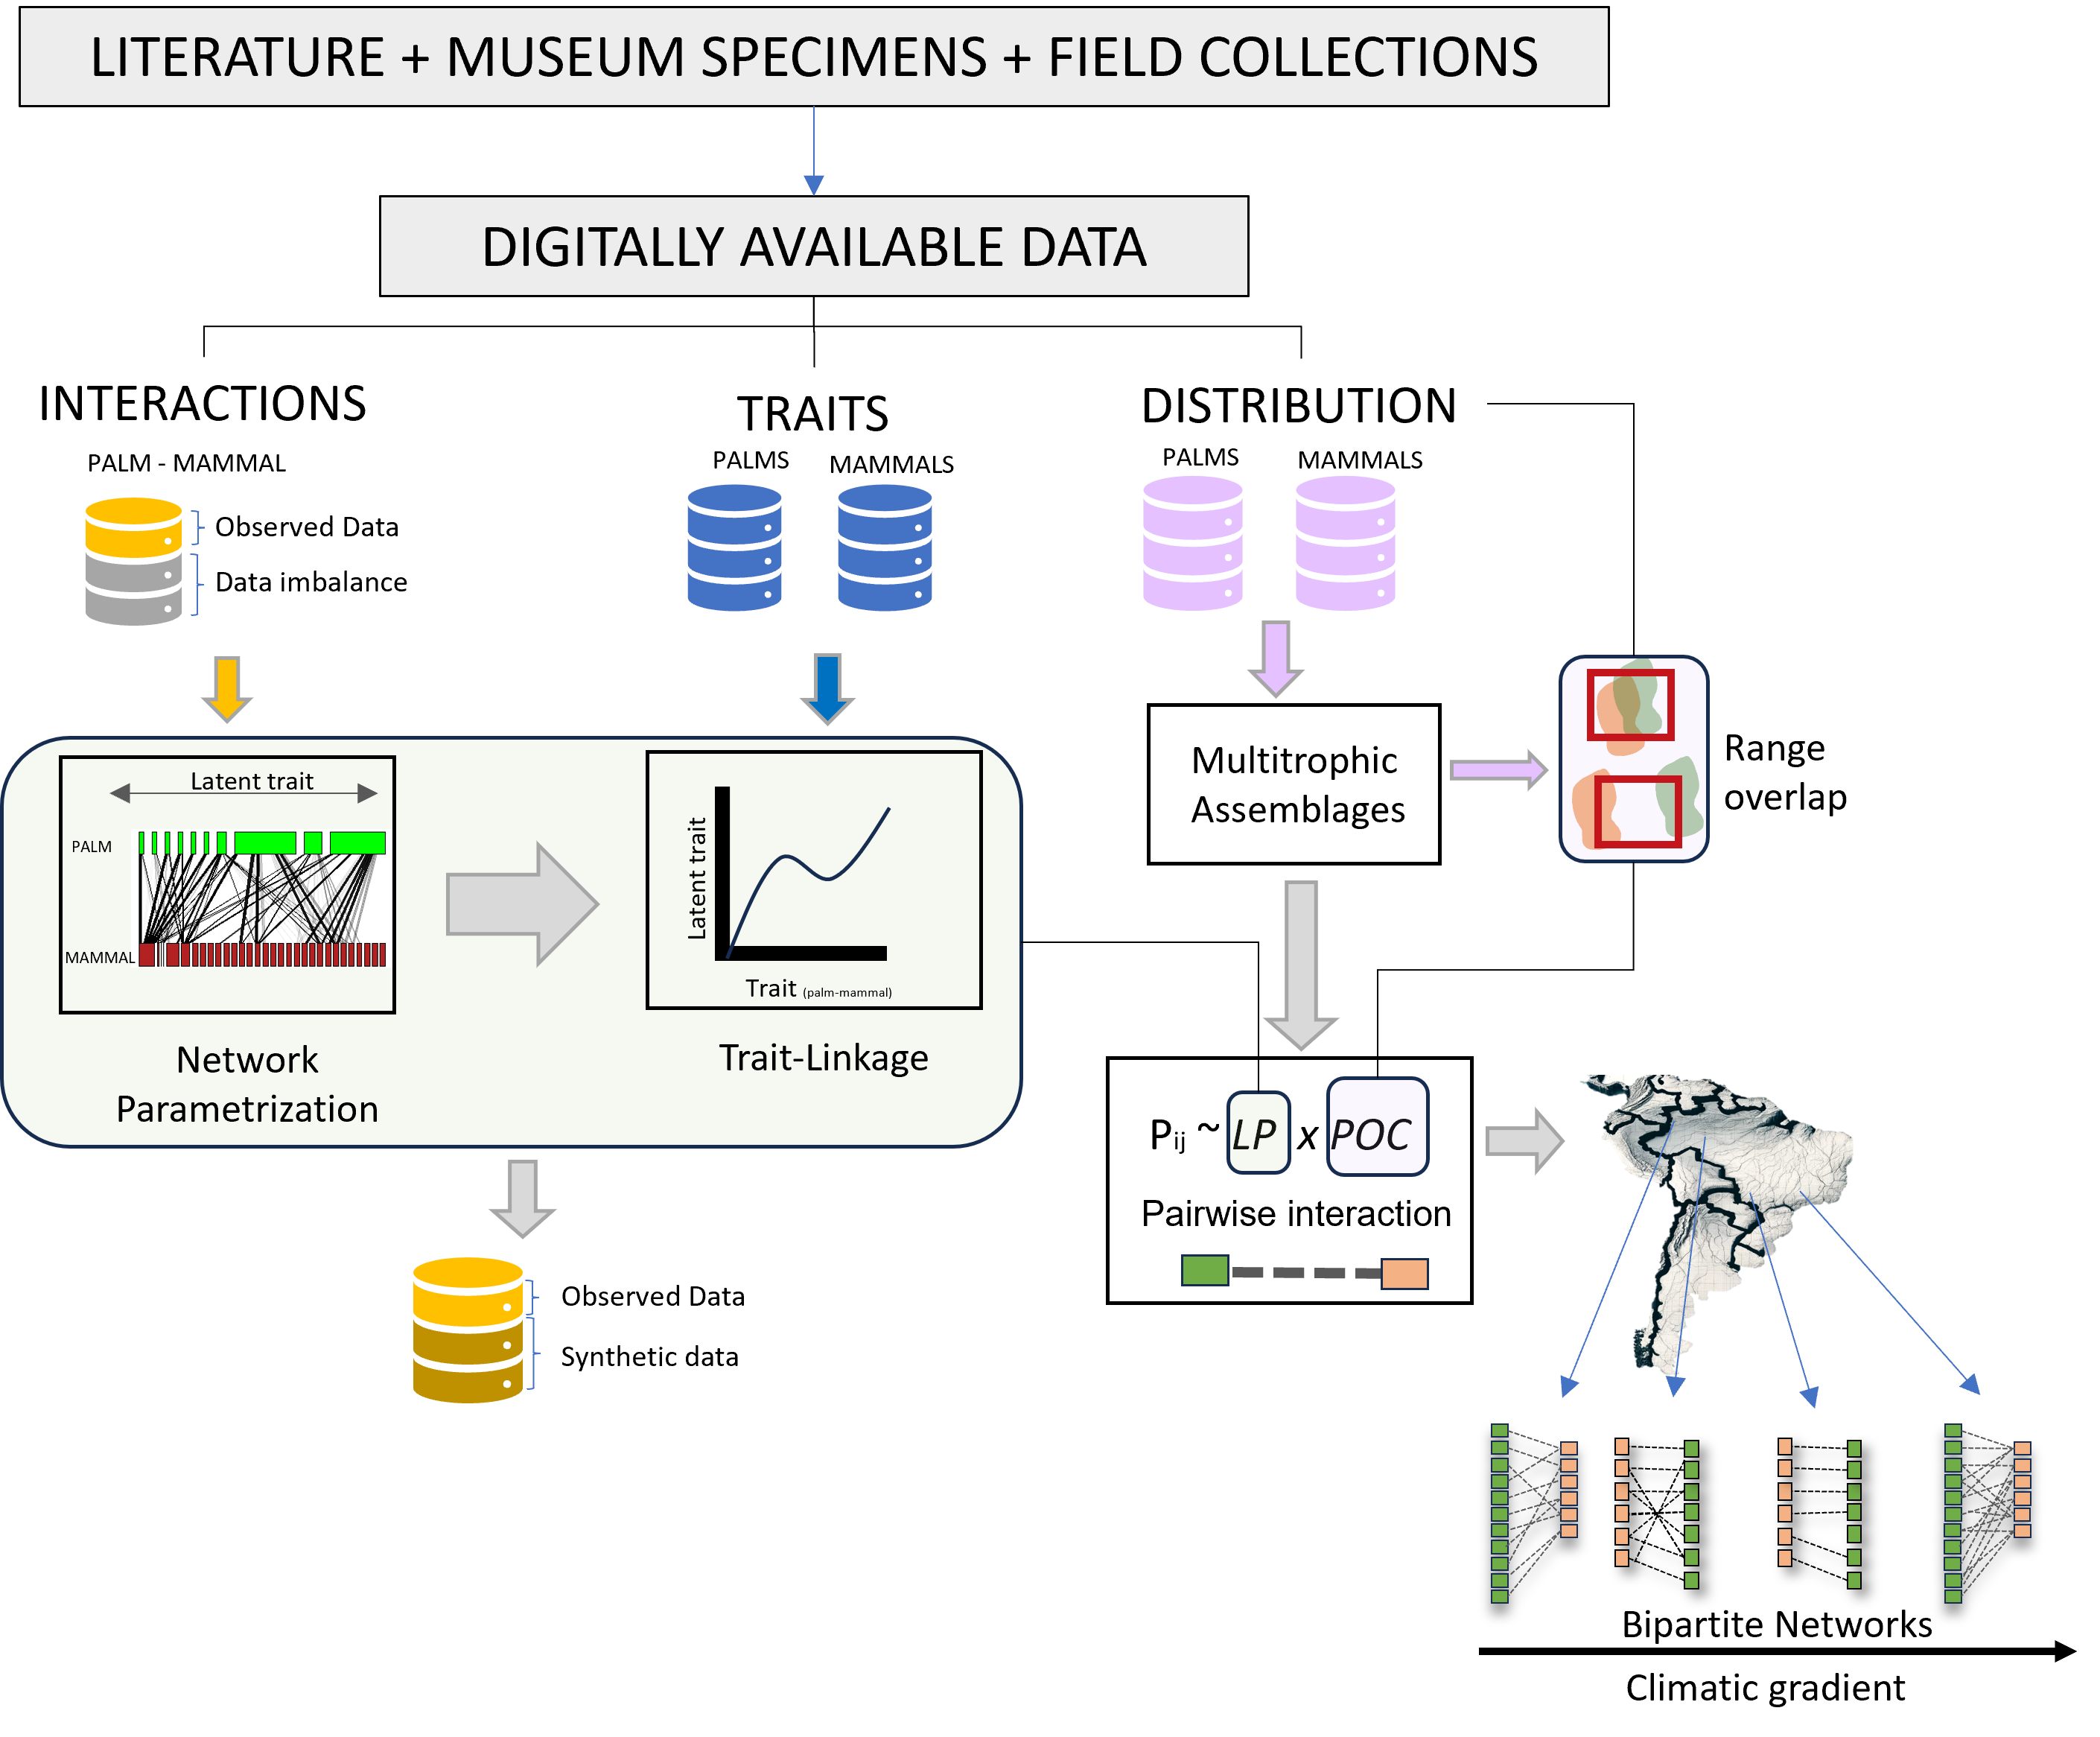
\includegraphics{Sup_figures/00_figure_data_pipeline.png}

}

\caption{Figure S1: A comprehensive workflow designed to integrate and
harmonize primary biodiversity data from digitally accessible datasets.
In our case study, these datasets are systematically categorized into
three key components: palm-mammal interactions, species traits, and
geographical distribution. The workflow is structured to address data
imbalances through network parametrization, which ensures that
underrepresented data is appropriately synthesized to generate a more
balanced dataset. Additionally, trait-linkage analysis is employed to
examine relationships between latent traits, facilitating a deeper
understanding of species interactions. Further, we examine the assembly
of multitrophic networks, which are constructed based on their matching
traits and the spatial overlap of species distributions. Ultimately,
these networks can provide insights on the drivers of network assembly
across diverse environmental gradients.}

\end{figure}%%
\begin{figure}[H]

{\centering 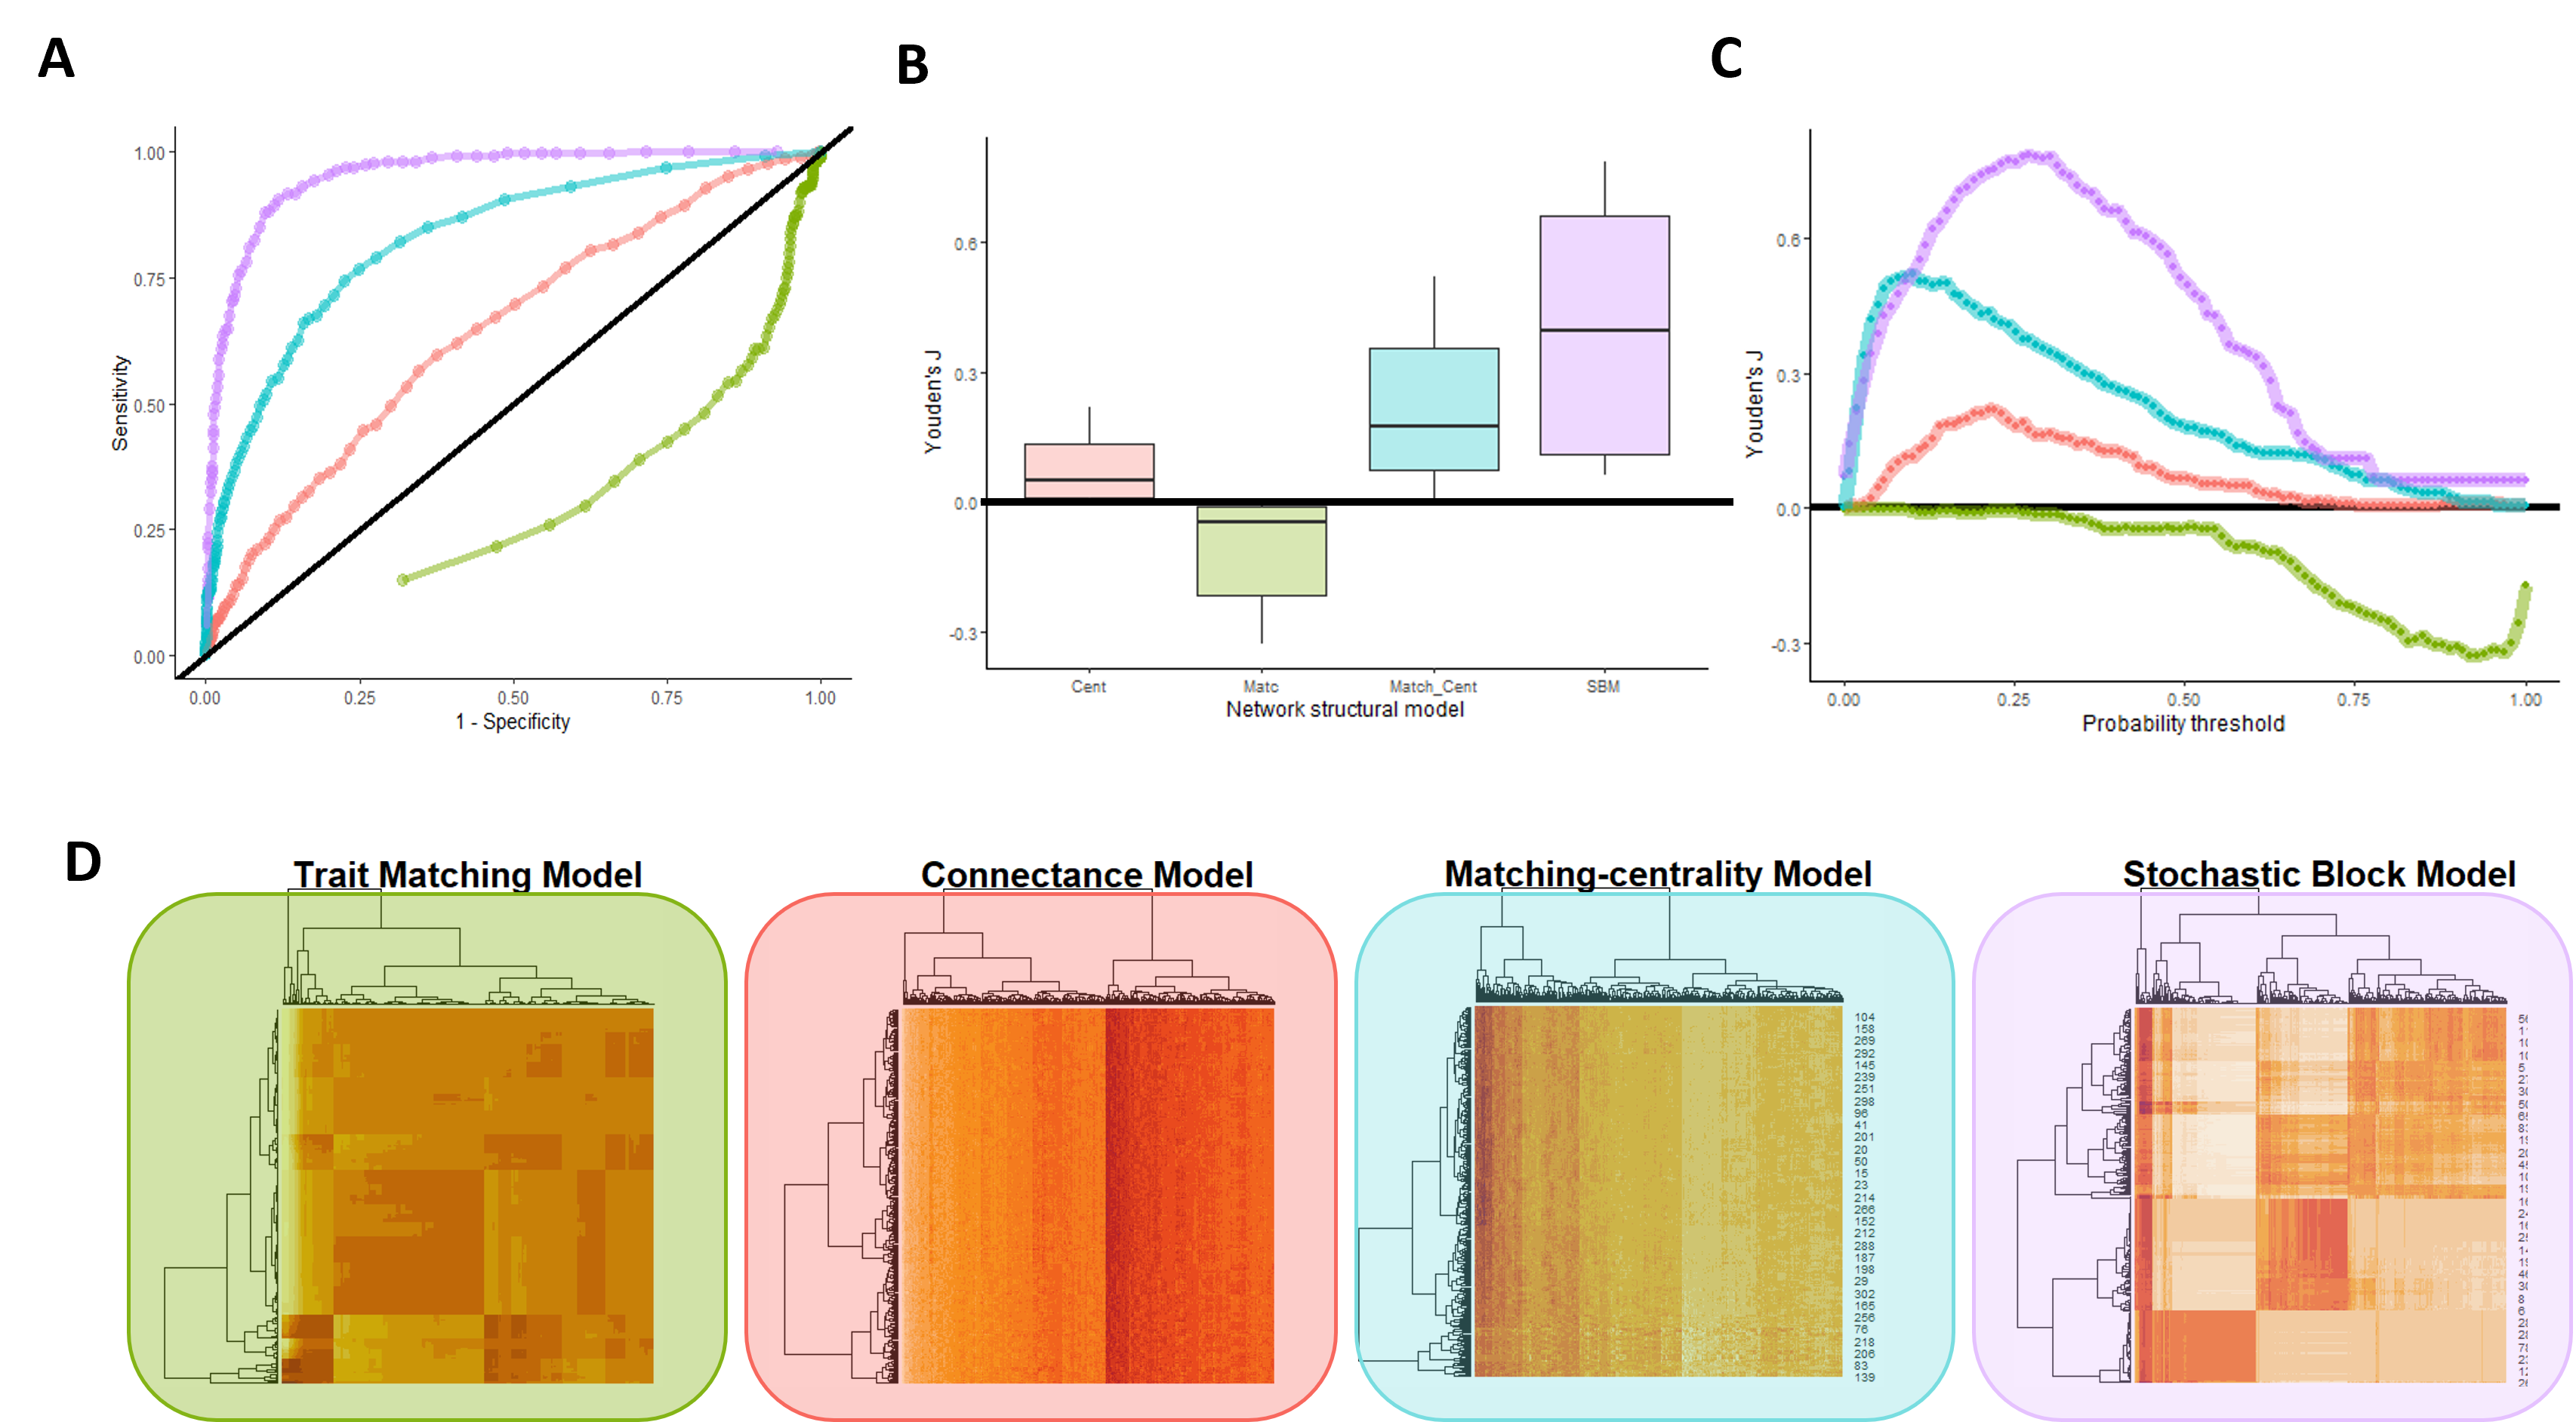
\includegraphics{Sup_figures/00_figure_data_metaweb_fit.png}

}

\caption{Figure S2: Evaluating distinct network structural models to
predict mutualistic interactions between palms and mammals in the
Neotropics. \textbf{(A) Receiver Operating Characteristic (ROC) Curves}:
This panel illustrates the performance of different network structural
models in predicting interactions across species pairs. Each curve is
color-coded to represent a distinct model, providing insight into the
trade-off between true positive and false positive rates across varying
thresholds. \textbf{(B) Boxplots of Model Accuracy}: This panel compares
the accuracy of the models, displaying the distribution of accuracy
scores across multiple datasets or iterative simulations. The
variability, indicated by the spread of the boxplots, highlights the
consistency and reliability of each model's predictions. \textbf{(C)
Precision-Recall (PR) Curves}: This panel focuses on the trade-offs
between precision and recall (evaluated with Youden's J) at different
probability thresholds for each model. The curves help to identify the
most effective models in minimizing false positives while maximizing
true positives, especially in imbalanced datasets such as ours where
interactions are sparse. \textbf{(D) Heatmaps of Predicted Adjacency
Matrices}: This panel visualizes the predicted interactions in the form
of adjacency matrices for the four distinct models examined in this
study: the Trait Matching Model, Connectance Model, Matching-centrality
Model, and Stochastic Block Model. Hierarchical clustering applied to
species based on their predicted interactions helps in elucidating the
structural differences between models, revealing patterns of species
clustering and potential interaction modules.}

\end{figure}%%
\begin{figure}[H]

{\centering 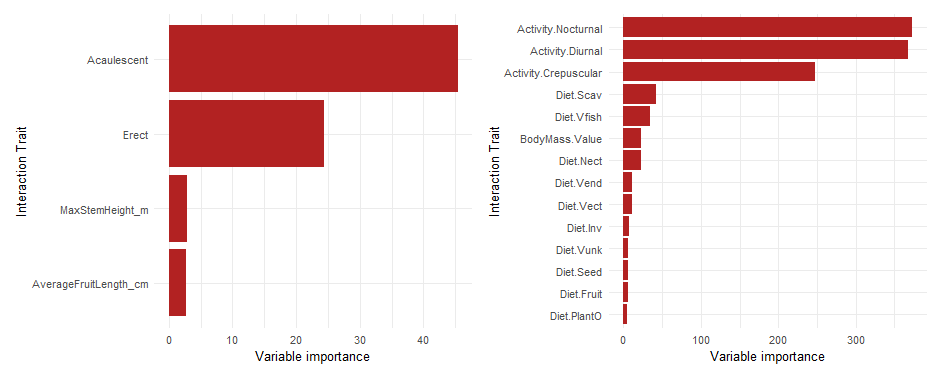
\includegraphics{Sup_figures/00_Variable_importance.png}

}

\caption{Figure S3: \textbf{Variable Importance for Interaction Traits
in Palm and Mammal frugivores}. The left panel presents the relative
importance of palm interaction traits, where \emph{Acaulecscent} and
\emph{Erect} growth forms are identified as the most influential traits
to define interactions with mammals. Secondary traits such as
\emph{MaxStemHeight\_m} and \emph{AverageFruitLength\_cm} contribute
moderately to delineate interactions. The right panel shows the
importance of mammal interaction traits in shaping their interactions
with palms, with activity patterns---nocturnal and diurnal---emerging as
the most critical. Crepuscular activity also shows notable relevance.
Among diet-related traits, scavenging and fish consumption, alongside
body mass, are recognized as important, though their influence is
comparatively lower.}

\end{figure}%%
\begin{figure}[H]

{\centering 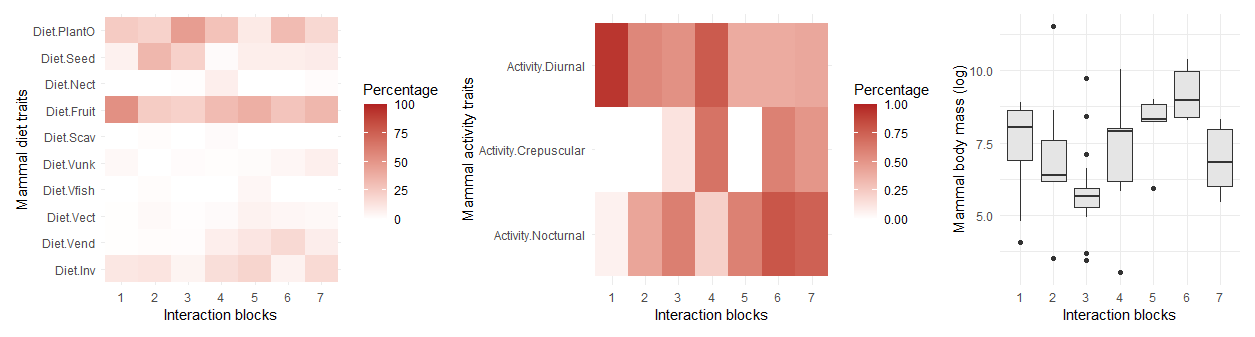
\includegraphics{Sup_figures/Trait_associations.png}

}

\caption{Figure S4: \textbf{Mammal trait representations across SBM
groups (interaction blocks).} \textbf{Dietary Traits (Left Panel):} The
heatmap illustrates the percentage distribution of various mammalian
diet types across the interaction blocks (SBM groups). Darker shades
indicate a higher prevalence of specific diet types within particular
blocks. This distribution reveals the trophic specialization of mammals
and suggests how different diet types are clustered or dispersed across
ecological interactions. \textbf{Activity Patterns (Middle Panel):} The
second heatmap focuses on mammalian activity data, categorized as
Diurnal, Crepuscular, and Nocturnal. Darker shades signify higher
percentages, allowing for a comparison of how activity patterns are
distributed across the same interaction blocks. This panel helps in
understanding temporal niche partitioning and its relationship to
ecological interactions. \textbf{Body Mass Variation (Right Panel):} The
boxplot illustrates the distribution of mammalian body mass
(log-transformed) across the interaction blocks.}

\end{figure}%%
\begin{figure}[H]

{\centering 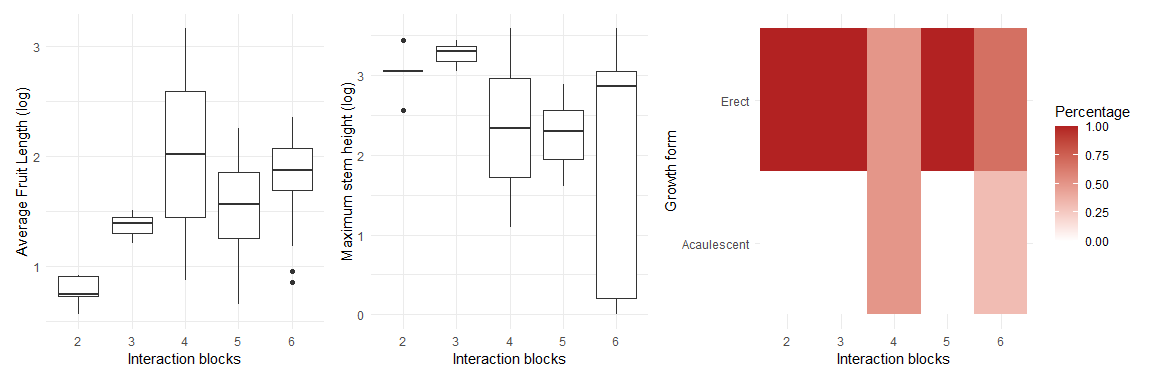
\includegraphics{Sup_figures/00_palm_trait_decomposition.png}

}

\caption{Figure S5: \textbf{Palm trait representations across SBM groups
(interaction blocks).} The left and middle panels feature boxplots that
display the log-transformed average fruit length and maximum stem
height, respectively, for each interaction block. The right panel shows
the relative proportions of plant growth forms within each interaction
block. The color gradient represents the percentage contribution of each
growth form.}

\end{figure}%%
\begin{figure}[H]

{\centering 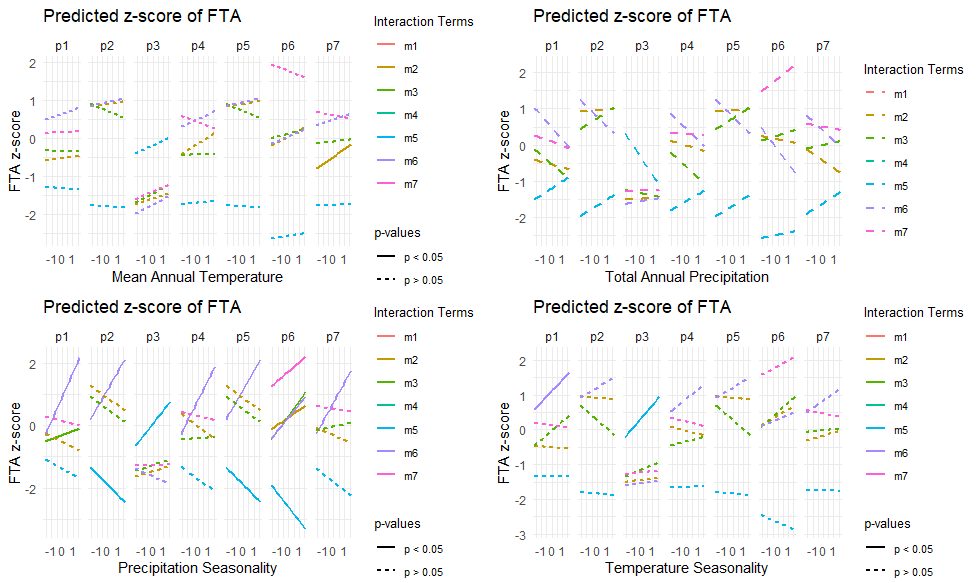
\includegraphics{Sup_figures/00_climate_effects.png}

}

\caption{Figure S6: \textbf{Predicted z-scores of FTA (Functional Trait
Assemblage) as a function of four climate variables and across
combinations of seven different palm (p1 to p7) and seven mammal (m1 to
m7) SBM groups}. The four panels represent: Mean Annual Temperature (top
left), Total Annual Precipitation (top right), Precipitation Seasonality
(bottom left), and Temperature Seasonality (bottom right). Solid lines
indicate statistically significant relationships (p \textless{} 0.05),
while dashed lines indicate non-significant relationships (p ≥ 0.05).
The different interaction models are color-coded as indicated in the
legend and the facet title.}

\end{figure}%%
\begin{figure}[H]

{\centering 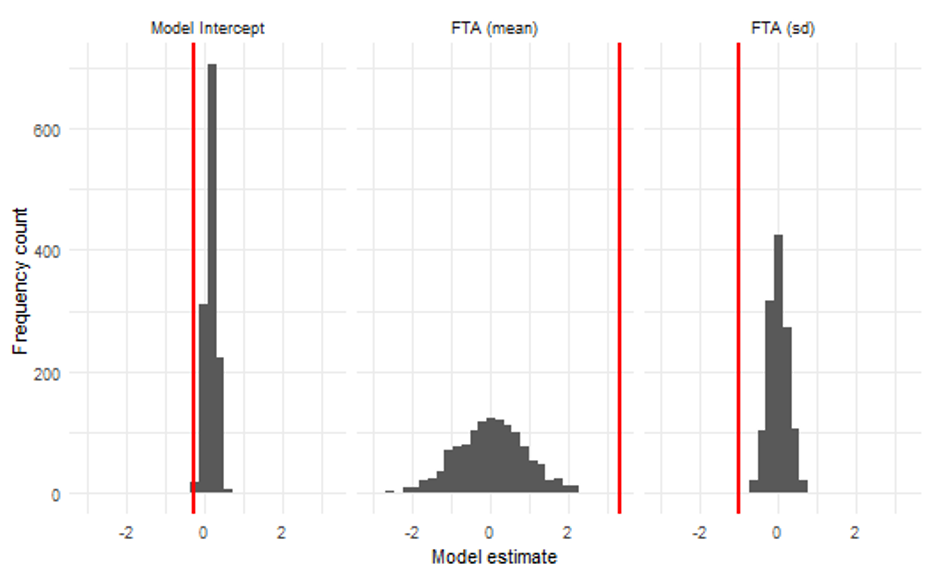
\includegraphics{Sup_figures/00_simulations_estimates.png}

}

\caption{Figure S7: \textbf{Frequency distribution of model estimates
for the intercept and Functional Trait Asymmetry (FTA) metrics}. The
three panels display the distribution of model estimates for the
intercept (left), FTA mean (center), and FTA standard deviation (right).
Red vertical lines denote the actual estimates obtained from the model,
serving as a reference point against the resampled or bootstrapped
estimate distributions. The histograms illustrate the frequency count of
estimates derived from a null model that reshuffled species
co-occurrences. FTA mean is the mean FTA z-scores for all SBM
palm-mammal group combinations in a gridcell. FTA sd is the standard
deviation of the distribution of FTA z-scores for all SBM palm-mammal
group combinations in a gridcell}

\end{figure}%

\subsection{Supplementary text}\label{supplementary-text}

\textbf{Supplementary text S1: Additional details about the structural
network models used to predict species interactions in this study}

To capture probabilistic patterns from interactions observed at the
continental scale, we tested four assembly models: the stochastic block
model (SBM), the connectance model, the matching-trait model, and the
matching-centrality model. Each model was evaluated based on its ability
to predict interaction probabilities between palm and mammal species
pairs.

\begin{itemize}
\item
  \textbf{1. Stochastic Block Model (SBM):}

  The SBM assumes that ecological networks exhibit a modular pattern,
  where subsets of species interact more within their groups of highly
  connected species (Terry and Lewis, 2020).
\end{itemize}

The model generates an incidence matrix, ( Z ), reflecting species-level
associations to a group, and a squared matrix, \(( \Theta )\),
reflecting the interaction probabilities within and between groups. The
likelihood ( L ) of the SBM is given by:

\[
L = \prod_{i,j} \left( \Theta_{Z_i Z_j} \right)^{A_{ij}} \left( 1 - \Theta_{Z_i Z_j} \right)^{1 - A_{ij}}
\]

where

\begin{itemize}
\item
  \(( A )\) is the adjacency matrix of observed interactions,
\item
  \(( Z_i) (Z_j)\) are the group memberships of species ( i ) and ( j ),
  and
\item
  \(( \Theta_{Z_i Z_j} )\) is the probability of interaction between
  groups ( Z\_i ) and ( Z\_j ).
\item
  \textbf{2. Connectance Model:}
\end{itemize}

The connectance model posits that the interactions of specialist species
are subsets of those of generalist species. It optimizes connectivity
scores, \(( C_i)\), assigned to species to maximize the likelihood of
recreating the observed network pattern. The likelihood ( L ) for this
model is:

\[
L = \prod_{i,j} \left( C_i \cdot C_j \right)^{A_{ij}} \left( 1 - C_i \cdot C_j \right)^{1 - A_{ij}}
\]

where \(( C_i)\) is the connectivity score of species \((i)\).

\begin{itemize}
\tightlist
\item
  \textbf{3. Matching-Trait Model:}
\end{itemize}

The matching-trait model assumes that species interactions are not
random but based on trait differences. It optimizes parameters by
scoring interactions along one or multiple latent-trait axes. The
interaction probability \(( P_{ij})\) between species ( i ) and ( j ) is
determined by:

\[
P_{ij} = f(T_i, T_j)
\]

where \(( T_i)\) and \(( T_j)\) are trait vectors for species ( i ) and
( j ), and ( f ) is a function measuring trait similarity or
compatibility.

\begin{itemize}
\tightlist
\item
  \textbf{4. Matching-Centrality Model:}
\end{itemize}

The matching-centrality model combines the approaches of the connectance
and matching-trait models. It optimizes both species connectivity scores
and latent trait axes. The likelihood ( L ) for this model is:

\[
L = \prod_{i,j} \left( C_i \cdot C_j \cdot f(T_i, T_j) \right)^{A_{ij}} \left( 1 - C_i \cdot C_j \cdot f(T_i, T_j) \right)^{1 - A_{ij}}
\]

Following the guidelines established by Poisot (2023), Youden's J
statistic was used to compare model performance. Youden's J is a metric
of model informedness that balances sensitivity and specificity,
calculated as:

\[
J = \text{Sensitivity} + \text{Specificity} - 1
\]

\section{Data Accessibility
Statement}\label{data-accessibility-statement}

Data is open-source, digitally available at their respective sources.

\section{Conflict of Interest
Statement}\label{conflict-of-interest-statement}

The authors declare no conflict of interest.



\end{document}
